%%%%%%%%%%%%%%%%%%%%%%%%%%%%%%%%%%%%%%%%%%%%%%%%%%%%%%%%%%%%%%%%%%%%%%
% Câu chưa có mã dạng — cần gắn %[..] rồi chuyển vào đúng file dạng
% Số câu: 62  (sinh tự động bởi tach_cau.py; từ nay thầy sửa trực tiếp file này)
%%%%%%%%%%%%%%%%%%%%%%%%%%%%%%%%%%%%%%%%%%%%%%%%%%%%%%%%%%%%%%%%%%%%%%

%%%%%%%%%%%%%%%% ĐÚNG/SAI %%%%%%%%%%%%%%%%

% nguồn: Lop_12_Hinh_hoc_Chuong_2
\begin{ex}%[ma:74b30a4f]
	%[2H2H2-3] 
	Trong không gian $Oxyz$, cho  hai véc-tơ $\vec{a}=\vec{i}+\vec{j}-2\vec{k}$ và $\vec{b}=-2\vec{i}+\vec{j}+4\vec{k}$.
	 \choiceTF
		{\True Tọa độ của  véc-tơ $\vec{a}$~là $(1;1;-2)$}
		{Tọa độ của véc-tơ $\vec{b}$~là $(-2;1;-4)$} 
		{\True Tọa  độ của véc-tơ $-2\vec{b}$~là $(4;-2;-8)$}
		{\True Tọa độ  của véc-tơ $\vec{u}=\vec{a}-2\vec{b}$~là $(5;-1;-10)$}
	\loigiai{ 
	\begin{itemchoice}
		 \itemch \textbf{Đúng}. Tọa độ của véc-tơ $\vec{a}$~là $(1;1;-2)$.
		\itemch \textbf{Sai}. Tọa  độ của véc-tơ $\vec{b}$~là $(-2;1;4)$.
		\itemch \textbf{Đúng}. Tọa độ của véc-tơ $-2\vec{b}$~là $(4;-2;-8)$. 
		\itemch \textbf{Đúng}. Tọa độ của  véc-tơ $\vec{u}=\vec{a}-2\vec{b}$~là $(5;-1;-10)$.
	\end{itemchoice}
	 }
\end{ex}

% nguồn: Lop_12_Hinh_hoc_Chuong_2
\begin{ex}%[ma:6d463d97]
	%[2H2H2-2] 
	Trong không gian $Oxyz$, cho tam giác $ABC$  có $A(1;2;3)$, $B(-1;-2;0)$, $C(-3;0;6)$.
	 \choiceTF
		{Tổng các hoành độ của ba  điểm $A,B,C$~là $x_A+x_B+x_C=3$}
		 {\True Tổng các tung độ của ba điểm $A,B,C$~là $y_A+y_B+y_C=0$}
		{Tổng  các cao độ của ba điểm $A,B,C$~là $z_A+z_B+z_C=3$}
		{\True Tọa độ trọng tâm $G$ của tam giác  $ABC$~là $(-1;0;3)$}
	\loigiai{ 
	\begin{itemchoice}
		\itemch \textbf{Sai}.  Tổng các hoành độ của ba điểm $A,B,C$~là $x_A+x_B+x_C=-3$.
		\itemch  \textbf{Đúng}. Tổng các tung độ của ba điểm $A,B,C$~là $y_A+y_B+y_C=0$.
		\itemch \textbf{Sai}.  Tổng các cao độ của ba điểm $A,B,C$~là $z_A+z_B+z_C=9$.
		\itemch \textbf{Đúng}. Tọa độ trọng  tâm $G$ của tam giác $ABC$~là $(-1;0;3)$.
	\end{itemchoice}
	} 
\end{ex}

% nguồn: Lop_12_Hinh_hoc_Chuong_2
\begin{ex}%[ma:d29accff]
	%[2H2V2-3] 
	Trong không gian, cho hình lập phương $ABCD.A'B'C'D'$ có  canh bằng~$a $.
	 \choiceTF
		{\True $|\overrightarrow{A'B'}-\overrightarrow{DC'}|=a$} 
		{$\overrightarrow{AB}=\overrightarrow{CD}$} 
		{$\overrightarrow{AB}\cdot  \overrightarrow{B'C'}=a^2$}
		{\True Gọi  $N$ là~điểm thỏa $\overrightarrow{C'N}=2\overrightarrow{NB'}$. Khi đó $\overrightarrow{AN}=\overrightarrow{AA'}+\overrightarrow{AB}+\dfrac{1}{3}\overrightarrow{AD}$}
	\loigiai{ 
		\par 
		\begin{tikzpicture}[>=stealth,line join=round,line cap=round,declare function={a=4;}]
				\draw[dashed] (0,0)  coordinate (A)--(-140:{0.6*a}) coordinate (B)
					(a,0) coordinate (D)--(A)--($(A)+(90:a)$) coordinate (A'); 
				\draw (B)--($(D)-(A)+(B)$)  coordinate (C)--(D)--($(D)+(90:a)$) coordinate (D')--(A')--($(B)+(90:a)$) coordinate (B')--($(D')-(A')+(B')$) coordinate (C')--(D')
					 (C')--(C)
					 (B')--(B);
				\path pic[angle  radius=5,angle eccentricity=1.5]{right angle = D--A--A'};
				\coordinate (N) at ($(B')!0.75!(C')$); 
				\draw [dashed] (A)--(N); 
				\foreach \diem/\vitrin in {A/left,B/below left,C/below right,D/right,A'/left,B'/below left,C'/below right,D'/right,N/above} \fill (\diem)  circle (1pt) node[\vitrin]{$\diem$};
			\end{tikzpicture}
		\begin{itemchoice}
			 \itemch \textbf{Đúng.}\\
			Ta  có$\overrightarrow{A'B'}-\overrightarrow{DC'}=\overrightarrow{DC}-\overrightarrow{DC'}=\overrightarrow{C'C} $.\\
			Suy ra $| \overrightarrow{A'B'}-\overrightarrow{DC'} |=|  \overrightarrow{C'C} |=a $.\\
			\itemch  \textbf{Sai}\\
			Vì$\overrightarrow{AB}=-\overrightarrow{CD} $.\\ 
			\itemch  \textbf{Sai}\\
			Vì$\overrightarrow{AB}\cdot \overrightarrow{B'C'}=\overrightarrow{AB}\cdot \overrightarrow{BC}=0$ (vì  $\overrightarrow{AB}\perp \overrightarrow{BC}$).\\
			\itemch \textbf{Đúng.}\\ 
			 Ta có$\overrightarrow{AN}=\overrightarrow{AB}+\overrightarrow{BB'}+\overrightarrow{B'N}=\overrightarrow{AB}+\overrightarrow{AA'}+\dfrac{1}{3}\overrightarrow{B'C'}=\overrightarrow{AB}+\overrightarrow{AA'}+\dfrac{1}{3}\overrightarrow{AD} $.
		\end{itemchoice}
	} 
\end{ex}

% nguồn: Lop_12_Hinh_hoc_Chuong_2
\begin{ex}%[ma:6a36b7ea]
	%[2H2V1-3] 
	Cho hình tứ diện $ABCD$ có $AB$, $AC$, $AD$ đôi một vuông góc, cạnh $AB = AC = a $, $M$ là~trung điểm của $CB$, $H$ là~trung điểm  của $MD$. Xét tính đúng sai các khẳng định sau.
	\choiceTF 
		{\True $\overrightarrow{DM} = \dfrac{1}{2}\left(\overrightarrow{DB} + \overrightarrow{DC}\right) $} 
		{Góc giữa $ \overrightarrow{AH} \text{ và } \overrightarrow{BC} \text{ bằng } 60^\circ $} 
		{\True  $ \overrightarrow{AB} \cdot \overrightarrow{AH} = \dfrac{a^2}{4} $}
		{\True $ \overrightarrow{AH} = \dfrac{1}{2}\cdot  \overrightarrow{AD} + \dfrac{1}{4}\left(\overrightarrow{AB} + \overrightarrow{AC}\right) $}
	\loigiai{ 
		\begin{center}
			\begin{tikzpicture}[line join=round,line cap=round,scale=0.6]
					 \tikzset{ethicknode/.style={scale=0.7}}
					\coordinate (A) at (0,0); 
					\coordinate (B) at  (-2,-3);
					 \coordinate (C) at (5,0);
					 \coordinate (G) at (1,-1.3);
					\coordinate (D) at ($(A)+(0,5)$); 
					\coordinate (M) at ($(B)!0.5!(C)$); 
					\coordinate (H) at ($(M)!0.5!(D)$); 
					\draw  (D)--(B)
						(D)--(C) 
						 (D)--(C)
						(C)--(B) 
						 (M)--(D);
					 \draw[dashed] (D)--(A)
						 (A)--(B)
						(A)--(C) 
						 (A)--(H)
						 (A)--(M);
					\pic[draw,thin,angle radius=3mm]{right angle =  D--A--C} pic[draw,thin,angle radius=3mm]{right angle = D--A--B} pic[draw,thin,angle radius=3mm]{right angle = B--A--C};
					\foreach \i/\g in {D/90,A/-90,B/-90,C/0,M/-90,H/40}{\fill (\i) circle (1pt) 
						($(\i)+(\g:3mm)$)  node[scale=1]{$\i$};}
				\end{tikzpicture}
		\end{center}
		\begin{itemchoice}
			 \itemch
			Vì $M$ là~trung điểm của $BC$ nên $\overrightarrow{DM} = \dfrac{1}{2}\left(\overrightarrow{DB} +  \overrightarrow{DC}\right)$
			 \itemch
			Vì tam  giác $ABC$ vuông cân tại $A$, ta có
			 \[
			AM \perp BC \quad  (1)
			\] 
			Mặt  khác
			 \[
			\begin{cases}
				 AD \perp AB \\
				AD \perp  AC
			\end{cases}
			\Rightarrow AD \perp (ABC)  \Rightarrow AD \perp BC \quad (2)
			\] 
			Từ $(1)$ và $(2)$ suy ra 
			\[ 
			BC \perp (AMD) \Rightarrow BC \perp AH \quad \text{ (do $AH \subset  (AMD)$)}
			 \]
			 Suy ra $(AH, BC) = 90^\circ$.
			 \itemch
			Ta  có $BC = AB \sqrt{2} = a \sqrt{2}, \quad AM = \dfrac{BC}{2} = \dfrac{a \sqrt{2}}{2}$.\\
			Vì $H$ là~trung điểm của $DM$ nên  $AH = \dfrac{1}{2} (\overrightarrow{AD} + \overrightarrow{AM})$.\\
			Khi đó 
			\begin{eqnarray*}
				\overrightarrow{AB}  \cdot \overrightarrow{AH} &=&\overrightarrow{AB} \cdot \dfrac{1}{2} (\overrightarrow{AD} + \overrightarrow{AM})=\dfrac{1}{2}\overrightarrow{AB}\cdot \overrightarrow{AD}+\dfrac{1}{2}\overrightarrow{AB}\cdot \overrightarrow{AM}\\
				&=& 
				 \dfrac{1}{2}\overrightarrow{AB}\cdot \overrightarrow{AM}\\
				 &=&\dfrac{1}{2} AB \cdot AM \cdot \cos 45^\circ\\
				 &=&\dfrac{1}{2} a \cdot \dfrac{a \sqrt{2}}{2} \cdot \dfrac{\sqrt{2}}{2}\\
				&=& \dfrac{a^2}{4}. 
			\end{eqnarray*}
			\itemch 
			 Vì $H$ là~trung điểm của $DM$ nên $ \overrightarrow{AH} = \dfrac{1}{2} (\overrightarrow{AD} + \overrightarrow{AM})$.
			Vì $M$  là~trung điểm của $BC$ nên $ \overrightarrow{AM} = \dfrac{1}{2} (\overrightarrow{AB} + \overrightarrow{AC})$.
			Khi đó 
			\[ 
			\overrightarrow{AH} =  \dfrac{1}{2}\left(\overrightarrow{AD} + \overrightarrow{AM}\right) = \dfrac{1}{2}\cdot \overrightarrow{AD} + \dfrac{1}{4}\left(\overrightarrow{AB} + \overrightarrow{AC}\right).
			 \]
		\end{itemchoice}
	} 
\end{ex}

% nguồn: Lop_12_Hinh_hoc_Chuong_2
\begin{ex}%[ma:e7ceb4a6]
	%[2H2V2-2] 
	Trong không gian với hệ tọa độ $Oxyz$, cho tam giác $ABC$ với $A(4;0;2)$, $B(1;-4;-2)$ và $C(2;1;1)$.  Khi đó
	\choiceTF 
		{\True  Tọa độ trọng tâm tam giác $ABC$ là~$G\left(\dfrac{7}{3};-1; \dfrac{1}{3} \right)$}
		{Điểm $D$ thỏa mãn $ABDC$ là~hình bình hành, khi đó tọa độ  điểm $D$ là~$D(5;5;5)$}
		{Tam giác $ABC$ là~tam giác tù} 
		{Gọi điểm $E(a;b;c)$ là~giao điểm của đường thẳng $BC$ với mặt phẳng tọa độ $(Oxz)$, khi đó  $\dfrac{2a}{c}+b=\dfrac{9}{2}$}
	 \loigiai{
		\begin{itemchoice}
			\itemch Tọa độ trọng tâm là~$G\left(\dfrac{4+1+2}{3};\dfrac{0+(-4)+1}{3};\dfrac{2+(-2)+1}{3} \right)=G\left(\dfrac{7}{3};-1;\dfrac{1}{3} \right)$. 
			\itemch Tứ giác  $ABDC$ là~hình bình hành khi và chỉ khi
			\[\overrightarrow{CD}=\overrightarrow{AB}\Leftrightarrow \heva{&x_D-2=-3\\&y_D-1=-4\\&z_D-1=-4}\Leftrightarrow  \heva{&x_D=-1\\&y_D=-3\\&z_D=-3.}\]
			Vậy $D(-1;-3;-3)$. 
			\itemch Ta  có $\overrightarrow{BC}=(1;5;3)$; $\overrightarrow{AC}=(-2;1;-1)$.\\
			Do đó $\overrightarrow{BC}\cdot \overrightarrow{AC}=-2+5-3=0$ nên tam giác $ABC$ vuông tại $C$. 
			 \itemch Vì $E$ thuộc mặt phẳng $Oxz$ nên $E(a;0;c)$.\\
			 Ta có $\overrightarrow{BE}=(a-1;4;c+2),\overrightarrow{BC}=(1;5;3)$.\\
			$E$ là~giao điểm của đường thẳng $BC$  với mặt phẳng $(Oxz)$.\\
			Suy ra $B$, $C$, $E$ thẳng hàng nên hai vectơ $\overrightarrow{BC}$, $\overrightarrow{BE}$ cùng phương,  do đó
			 \[\overrightarrow{BE}=k\overrightarrow{BC}\Leftrightarrow \heva{&a-1=k\\&4=5k\\&c+2=3k}\Leftrightarrow \heva{&a=\dfrac{9}{5}\\&k=\dfrac{4}{5}\\&c=\dfrac{2}{5}.}\]
			 Suy ra $E\left(\dfrac{9}{5};0;\dfrac{2}{5} \right)\Rightarrow \dfrac{2a}{c}+b=9$.
		\end{itemchoice}
	} 
\end{ex}

% nguồn: Lop_12_Hinh_hoc_Chuong_2
\begin{ex}%[ma:e9c37515]
	 %[2H2V2-6]
	Trong không gian với hệ trục $Oxyz$ (đơn vị trên mỗi  trục là~1 m), một flycam bay với vận tốc có độ lớn và hướng không đổi. Tại thời điểm $t=0$, flycam ở vị trí $A(1; 2; 3)$ và sau $10$ phút nó ở vị trí $B(21; 32; 33)$.
	 \choiceTF
		{Flycam không bay qua vị trí $D(5; 8; 9)$} 
		{vectơ  vận tốc của flycam có tọa độ là~$\overrightarrow{v}=(20; 30; 30)$}
		{\True Độ lớn của vận  tốc flycam là~$\sqrt{22}$ (m/phút)}
		{\True Sau $15$ phút vị trí flycam là~$C(31;  47; 48)$}
	 \loigiai{
		\begin{itemchoice}
			 \itemch
			$\overrightarrow{AB}=(20; 30; 30)$; $\overrightarrow{AD}=(4; 6; 6)$.\\ 
			Ta có  $\dfrac{20}{4}=\dfrac{30}{6}=\dfrac{30}{6}$.\\
			Suy ra $\overrightarrow{AB}$, $\overrightarrow{AD}$  cùng phương\\
			$ \Rightarrow  $ 3 điểm $A$, $B$, $D$ thẳng hàng.\\
			Do đó flycam bay qua vị  trí $D(5; 8; 9)$.
			 \itemch
			Flycam ở vị trí $A(1; 2;  3)$ và sau 10 phút nó ở vị trí $B(21; 32; 33)$ \\
			$ \Rightarrow\overrightarrow{AB}=10\overrightarrow{v} $$ \Leftrightarrow\overrightarrow{v}=\dfrac{\overrightarrow{AB}}{10}=(2; 3; 3) $. 
			\itemch 
			Độ lớn của vận tốc flycam  là~$\left|\overrightarrow{v}\right|=\sqrt{2^2+3^2+3^2}=\sqrt{22}$ (m/phút).
			\itemch 
			Tại thời điểm $t=0$, flycam ở vị trí $A$ và sau 15 phút flycam ở vị trí  $C$.\\
			Suy ra $\overrightarrow{AC}=15\overrightarrow{v} \Leftrightarrow\left(x_C-1; y_C-2; z_C-3\right)=15(2; 3; 3)\Leftrightarrow \heva{&x_C=31\\&y_C=47\\&z_C=48.}  $\\
			 Vậy $C(31; 47; 48)$.
		\end{itemchoice}
	} 
\end{ex}

% nguồn: Lop_12_Hinh_hoc_Chuong_2
\begin{ex}%[ma:8ab2019f]
	%[2H2V2-6] 
	\immini{Hình vẽ sau mô tả vị trí của máy bay vào thời điểm $9h30$  phút. Biết các đơn vị tính theo đơn vị km.
	\choiceTF 
		 {\True Máy bay đang ở độ cao $9$ km}
		{\True Tọa độ của máy bay lúc $9h30$  là~$(150;300;9)$}
		{Phi công để máy bay ở chế độ tự động và bay theo hướng đông,  độ cao không đổi lúc 10h30 máy bay ở tọa độ $(150;1086;9)$. Khi đó vận tốc của máy bay là~$776$ km/h, biết vận tốc gió theo hướng đông là~$10$ m/s}
		{Giả sử vận tốc và hướng gió không đổi thì sau khi bay đến vị trí lúc 10h30 thì máy bay bay ngược lại (hướng Tây) với vận tốc $800$ km/h với  độ cao không đổi biết lúc đó trời lặng gió thì lúc $11$ giờ máy bay cách gốc tọa độ một khoảng $723$ km (làm tròn đến hàng đơn vị)}
		}{\resizebox{!}{5cm}{\begin{tikzpicture}[join = round,cap = round,>=stealth]
		 \path
			(0:0) coordinate  (D)
			 +(0:5) coordinate (C)
			+(65:3) coordinate  (O)
			($(O)  + (0,4)$) coordinate (E)
			($(O)+(C)-(D)$) coordinate (B) 
			($(E)+(C)-(O)$) coordinate (F) node{\Large  \faPlane}
			 ($(O)!1.2!(D)$) coordinate (M)
			($(O)!1.2!(B)$)  coordinate (N)
			 ($(O)!1.2!(E)$) coordinate (K);
		\foreach  \x/\y/\t in {O/M/x,O/N/y,O/K/z}
		 \draw[->]
			(\x)--(\y) node[right]{$\t$}; 
		\draw[dashed] 
			(E) -- (F)  --(C)
			(O)--(C) 
			(D)--(C)--(B); 
		\foreach  \x/\g/\t in {D/180/150,O/180/O,B/90/300,E/180/9}
		\fill (\x) circle (1pt) 
			node[shift={(\g:10pt)}]{$\t$}; 
		\foreach \x/\y/\z in {O/E/F,O/D/C,O/B/C}{ 
			\draw[thin] pic[draw,angle radius = 6pt]{right angle = \x--\y--\z}; 
		 }
	\end{tikzpicture}
		 }
		} 
	\loigiai{ 
		\begin{itemchoice}
			\itemch Máy bay đang ở độ cao  $9$ km.
			\itemch Toạ  độ của máy bay lúc 9h30 là~$(150;300;9)$
			\itemch $10  m/s = 36km/h$
			Gọi $A$ là~vị trí của máy bay lúc  9h30$ \Rightarrow A(150;300;9)$. \\
			Gọi $B$ là~vị trí của  máy bay lúc 10h30 $\Rightarrow B(150;1086;9)$. \\
			Quãng  đường máy bay di chuyển được từ 9h30 đến 10h30 là: $AB=\sqrt{0^2+786^2+0^2}=786km$ \\
			Khi đó vận tốc của máy  bay là: $786-36=750km/h$.
			\itemch Quãng đường máy  bay di chuyển được từ 10h30 đến 11 giờ là: $800 \cdot \dfrac{1}{2}=400$ km. \\
			Tại thời điểm $11$  giờ tọa độ máy bay là: $(150;686;9)$. \\
			Khoảng cách của  máy bay so với gốc tọa độ là: $\sqrt{150^2+686^2+9^2} \approx 702{,}3$ km/h.
		\end{itemchoice}
	 }
\end{ex}

% nguồn: Lop_12_Hinh_hoc_Chuong_2
\begin{ex}%[ma:b3bd5a24]
	 %[2H2H2-2]
	Trong không gian $Oxyz$, cho ba điểm $A(5;1;3)$, $B(1;6;2)$,  $C(5;0;4)$. Điểm $D$ thỏa mãn $ABCD$~là hình bình hành
	 \choiceTF
		 {$\overrightarrow{AB}=\overrightarrow{CD}$}
		{\True $\overrightarrow{AB}=(-4;5;-1)$} 
		{Nếu $D\left(x_0;y_0;z_0\right)$  thì $\overrightarrow{DC}=\left(x_0-5;y_0;z_0-4\right)$}
		{\True Tọa độ của điểm $D$~là  $(9;-5;5)$}
	 \loigiai{
	Gọi $D\left(x_0;y_0;z_0\right)$ thì $\overrightarrow{DC}=\left(5-x_0;-y_0;4-z_0\right)$  và $\overrightarrow{AB}=(-4;5;-1)$.\\
	Vì điểm $D$ thỏa  mãn $ABCD$~là hình bình hành nên
	$$\overrightarrow{DC}=\overrightarrow{AB} \Leftrightarrow  \heva{& 5-x_0=-4 \\ & -y_0=5 \\ & 4-z_0=-1} \Leftrightarrow \heva{& x_0=9 \\ & y_0=-5 \\ & z_0=5.}$$
	Vậy tọa~độ của điểm  $D$~là $(9;-5;5)$.
	\begin{itemchoice}
		\itemch \textbf{Sai}. 
		 \itemch \textbf{Đúng}.
		\itemch \textbf{Sai}. 
		 \itemch \textbf{Đúng}.
	\end{itemchoice}
	 }
\end{ex}

% nguồn: Lop_12_Hinh_hoc_Chuong_2
\begin{ex}%[ma:a789e82f]
	 %[2H2V1-1]
	Cho hình lập phương $ABCD. A'B'C'D'$ có cạnh bằng $a$. Gọi $I$ là~tâm hình vuông  $ABCD$, gọi $G$ là~trọng tâm của tam giác $AB'C$ (tham khảo hình vẽ).
	\begin{center}
		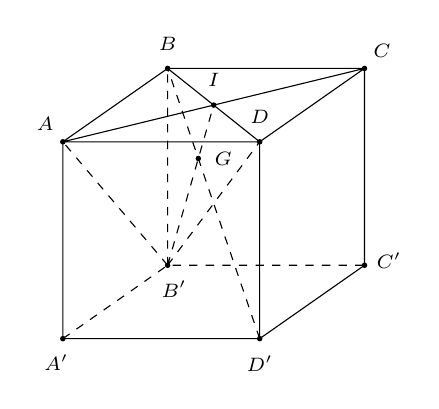
\begin{tikzpicture}[declare function={r=2.5;},font=\scriptsize]
				\path (0:0) coordinate (A) 
					(0:r) coordinate  (D)
					++(35:{0.65*r})  coordinate (C)
					 ++(180:r) coordinate (B)
				\foreach  \x in {A,B,C,D}{(\x)++(90:r) coordinate (\x_1)};
				\path (intersection of A_1--C_1  and B_1--D_1) coordinate (I);
				 \path (barycentric cs:B=1,B_1=1,D_1=1) coordinate (G);
				 \draw[dashed](A)--(B)--(C)
					(B)--(B_1) 
					(B)--(A_1) 
					 (D)--(B_1)
					(B)--(D_1) 
					 (B)--(I);
				\draw  (A)--(A_1)
					 (D_1)--(D)--(A)
					(D)--(C) 
					(C)--(C_1) 
					 (A_1)--(B_1)--(C_1)--(D_1)--cycle
					 (A_1)--(C_1)
					 (B_1)--(D_1);
				\foreach \x/\goc/\t in {A/255/A',B/-75/B',C/10/C',D/-90/D',A_1/135/A,B_1/90/B, 
					C_1/45/C,D_1/90/D,I/90/I,G/0/G}{ 
					\fill (\x)  circle (1pt) node[shift={(\goc:9pt)}]{$\t$};
				} 
			\end{tikzpicture}
	\end{center}
	\choiceTF 
		 {$\overrightarrow{GA}+\overrightarrow{GB'}+\overrightarrow{GC}=2\overrightarrow{GI}$}
		{\True $\overrightarrow{AB}+\overrightarrow{AD}+\overrightarrow{AA'}=\overrightarrow{AC'}$} 
		 {\True $\overrightarrow{AB}\cdot\overrightarrow{DD'}=0$}
		 {$\left(\overrightarrow{AC},\overrightarrow{DC'}\right)=30^{\circ}$}
	 \loigiai{
		\begin{itemchoice}
			\itemch Ta có  $\overrightarrow{GA}+\overrightarrow{GB'}+\overrightarrow{GC}=\left(\overrightarrow{GA}+\overrightarrow{GC}\right)+\overrightarrow{GB'}=2\overrightarrow{GI}+\overrightarrow{GB'}=\overrightarrow0$.
			Do đó ý a) \textbf{sai}. 
			\itemch Ta có $\overrightarrow{AB}+\overrightarrow{AD}+\overrightarrow{AA'}=\overrightarrow{AC'}$ (quy tắc hình hộp). Do đó ý b) \textbf{đúng}. 
			\itemch Ta có $\overrightarrow{AB}\cdot\overrightarrow{DD'}=\overrightarrow{DC}\cdot\overrightarrow{DD'}=0$ (vì $\overrightarrow{DC}\perp \overrightarrow{DD'}$).  Do đó ý c) \textbf{đúng}.
			\itemch Ta có $\left(\overrightarrow{AC},\overrightarrow{DC'}\right)=\left(\overrightarrow{AC},\overrightarrow{AB'}\right)=\widehat{CAB'}=60^{\circ}$ (vì $\triangle CAB'$ đều).  Do đó ý d) \textbf{sai}.
		\end{itemchoice}
	} 
\end{ex}

% nguồn: Lop_12_Hinh_hoc_Chuong_2
\begin{ex}%[ma:59f13f5f]
	 %[2H2H2-5]
	Trong không gian $Oxyz$, cho hai  véc-tơ $\vec{a}=(2;1;-3)$ và $\vec{b}=(-4;-2;6)$.
	 \choiceTF
		{\True  $\vec{b}=-2\vec{a}$}
		{\True $\left|\vec{b}\right|=2\left|\vec{a}\right|$} 
		 {\True $\left[\vec{a},\vec{b}\right]=\overrightarrow{0}$}
		{$\vec{a}$  cùng hướng với $\vec{b}$}
	 \loigiai{
	\begin{itemchoice}
		\itemch \textbf{Đúng}. Ta có $\vec{b}=-2\vec{a}$. 
		\itemch \textbf{Đúng}. Vì $\vec{b}=-2\vec{a}$ nên  $\left|\vec{b}\right|=2\left|\vec{a}\right|$.
		\itemch \textbf{Đúng}. Vì $\vec{a}$ và $\vec{b}$ cùng phương nên  $\left[\vec{a},\vec{b}\right]=\overrightarrow{0}$.
		\itemch \textbf{Sai}. Vì $\vec{b}=-2\vec{a}$ nên hai véc-tơ  này ngược hướng nhau.
	\end{itemchoice}
	} 
\end{ex}

% nguồn: Lop_12_Hinh_hoc_Chuong_2
\begin{ex}%[ma:db660381]
	%[2H2H2-3] 
	Trong không gian $Oxyz$,  cho hình hộp $ABCD.A'B'C'D'$ có $A(0;0;0)$, $B(1;-2;3)$, $D(-1;5;-2)$, $A'(-1;-2;0)$.
	\choiceTF 
		{\True $\overrightarrow{AB}=(1;-2;3)$} 
		{\True  $\overrightarrow{AD}=(-1;5;-2)$}
		{\True $\overrightarrow{AA'}=(-1;-2;0)$} 
		{Tọa  độ điểm $C'$~là $(1;-1;-1)$}
	 \loigiai{
		\begin{center}
			\resizebox{!}{5cm}{\begin{tikzpicture}[line join=round,line cap=round]
		 \path
			(0,0) coordinate (A) 
			(4,0)  coordinate (B)
			(-1.5,-1.5) coordinate (D) 
			($(B)+(D)-(A)$) coordinate (C) 
			($(A)!0.5!(C)$)  coordinate (O)
			($(O)+(0,5)$)  coordinate (A')
			($(A')+(B)-(A)$) coordinate  (B')
			($(A')+(C)-(A)$) coordinate  (C')
			($(A')+(D)-(A)$)  coordinate (D');
		\draw (B)--(C)--(D) 
			(A')--(B')--(C')--(D')--(A') 
			 (B)--(B')
			(C)--(C') 
			(D)--(D'); 
		\draw[dashed](B)--(A)--(D) 
			(A')--(A); 
		 \foreach \x/\g in{A/150,B/0,C/-90,D/-90,A'/90,B'/0,C'/0,D'/180}
		\fill (\x) circle  (1pt)
			($(\x)+(\g:3mm)$)  node{$\x$};
	\end{tikzpicture}
			} 
		\end{center}
		\begin{itemchoice}
			 \itemch \textbf{Đúng}. Ta có $\overrightarrow{AB}=(1;-2;3)$.
			\itemch  \textbf{Đúng}. Ta có $\overrightarrow{AD}=(-1;5;-2)$.
			\itemch \textbf{Đúng}.  Ta có $\overrightarrow{AA'}=(-1;-2;0)$.
			\itemch \textbf{Sai}. Xét hình bình hành  $ABCD$ ta có
			\[\overrightarrow{AD}=\overrightarrow{BC} \Rightarrow C(0;3;1).\] 
			Xét  hình bình hành $ACC'A'$ ta có
			\[\overrightarrow{AA'}=\overrightarrow{CC'} \Rightarrow  C'(-1;1;1).\]
		\end{itemchoice}
	} 
\end{ex}

% nguồn: Lop_12_Hinh_hoc_Chuong_2
\begin{ex}%[ma:475b2071]
	 %[2H2N2-2]%[2H5H1-5]
	\immini[thm]{Trong không gia $Oxyz$, cho hình lập phương $ABCD.A'B'C'D'$ có $A(0;0;0)$, $B(2;0;0)$, $D(0;2;0)$, $A'(0;0;2)$. Gọi  $M$, $N$ lần lượt~là trung điểm của $AB$ và $AA'$ (tham khảo hình vẽ).
	 \choiceTF
		{\True Toạ  độ của điểm $M$~là $(1;0;0)$}
		 {Toạ độ của điểm $N$~là $(0;1;0)$}
		{Phương trình  mặt phẳng $(DMN)$~là $\frac{x}{1}~=~\frac{y}{2}~=~\frac{z}{1}$}
		{\True  Khoảng cách từ điểm $C'$ đến mặt phẳng $(DMN)$ bằng~$\frac{8}{3}$}
		 }{
		\begin{tikzpicture}[font=\footnotesize,line join=round,line cap=round]
				\def\a{1} 
				\path (0:0) coordinate  (A)
					 (0:2.5*\a) coordinate (D)
					 ($(D)+(0:10mm)$) coordinate (y)
					(215:1.5*\a)  coordinate (B)
					($(B)+(215:10mm)$) coordinate  (x)
					 ($(B)+(D)-(A)$) coordinate (C)
					 ($(A)+(90:2.5*\a)$) coordinate (A')
					($(A')+(90:10mm)$) coordinate  (z)
					 ($(B)+(90:2.5*\a)$) coordinate (B')
					($(C)+(90:2.5*\a)$) coordinate  (C')
					($(D)+(90:2.5*\a)$) coordinate (D') 
					($(A)!1/2!(B)$) coordinate (M) 
					($(A)!1/2!(A')$) coordinate (N); 
				\draw[dashed] (B)--(A)--(D) 
					(A)--(A'); 
				\draw (C)--(C') 
					 (D)--(D')
					 (B)--(B')
					 (B)--(C)--(D)
					 (A')--(B')--(C')--(D')--cycle;
				\foreach \x/\pos in {A/45,B/160,C/-30,D/40,A'/160,B'/160,C'/-30,D'/30,M/160,N/1600} \fill  (\x) circle (1pt) node[{shift=(\pos:0.25)}]{$\x$};
				\foreach \x/\pos in {z/180,x/180,y/-9} \node[{shift=(\pos:0.25)}]  at (\x) {$\x$};
				\foreach \x/\y  in {B/x,D/y,A'/z}{\draw[-stealth] (\x)--(\y);}
				 \draw[dashed] (D)--(M)--(N)--cycle;
			\end{tikzpicture}
		} 
	\loigiai{ 
		\begin{itemchoice}
			\itemch \textbf{Đúng}.  Toạ độ của điểm $M$~là $(1;0;0)$.\\
			Ta có $\heva{&A(0;0;0)\\  &B(2;0;0)}$, $M$~là trung điểm $AB \Rightarrow M(1;0;0)$.
			\itemch \textbf{Sai}. Toạ độ của  điểm $N$~là $(0;1;0)$.\\
			Ta có $\heva{&A(0;0;0)\\ &A'(0;0;2)}$, $N$~là trung  điểm $AA' \Rightarrow N(0;0;1)$.
			\itemch \textbf{Sai}. Phương trình mặt phẳng $(DMN)$~là  $\dfrac{x}{1}~=~\dfrac{y}{2}~=~\dfrac{z}{1}$.\\
			 Phương trình $\dfrac{x}{1}=\dfrac{y}{2}=\dfrac{z}{1}$~là một phương trình chính tắc của một đường thẳng nào đó, không phải của mặt phẳng $(DMN)$.
			 \itemch \textbf{Đúng}. Khoảng cách từ điểm $C'$ đến mặt phẳng $(DMN)$ bằng $\dfrac{8}{3}$.\\
			Ta viết phương  trình mặt phẳng $(DMN)$.\\
			Cặp vectơ chỉ phương $\heva{\overrightarrow{DM}&=(1;-2;0)\\ \overrightarrow{DN}&=(0;-2;1)}$\\ 
			vectơ pháp tuyến  $\vec{n}=\left[\overrightarrow{DM},\overrightarrow{DN}\right]
			 =\left(
			\begin{vmatrix}
				-2 & 0 \\ -2 &  1
			\end{vmatrix};
			\begin{vmatrix}
				0 & 1  \\ 1 & 0
			\end{vmatrix};
			\begin{vmatrix}
				1 & -2 \\ 0 & -2 
			\end{vmatrix}
			\right)  =(-2;-1;-2)$.\\
			Ta có $(DMN)\colon -2(x-0)-1(y-2)-2(z-0) \Leftrightarrow 2x+y+2z-2=0$.\\ 
			Tứ giác $ABCD$~là  hình bình hành $ \Rightarrow C(2;2;0)$.\\
			Hình khối $ABCD.A'B'C'D'$~là hình lập phương $  \Rightarrow C'(2;2;2)$.\\
			Khoảng cách  $\mathrm{d}(C',(DMN))=\dfrac{\left|2\cdot2+1\cdot2+2\cdot2-2\right|}{\sqrt{2^2+1^2+2^2}}=\dfrac{8}{3}$.
		\end{itemchoice}
	 }
\end{ex}

% nguồn: Lop_12_Hinh_hoc_Chuong_2
\begin{ex}%[ma:23607e3f]
	 %[2H2H2-6]
	Hình vẽ  sau mô tả vị trí của máy bay vào thời điểm $9$ giờ $30$ phút. Biết các đơn vị trên hình tính theo đơn vị km. Mặt phẳng $(Oxy)$ trùng với mặt đất, $O$ trùng với vị trí trung tâm điều khiển.\\
	\begin{center}
		\resizebox{!}{5cm}{\begin{tikzpicture}[line join = round,line cap=round,>=stealth]
		 \path
			(0,0)  coordinate (O)
			(5,0) coordinate (B)  node[above]{$300$}
			(-3,-2) coordinate  (A) node[above left]{$150$}
			 (0,4) coordinate (C) node[above left]{$9$}
			 ($(A)+(B)-(O)$) coordinate (N)
			 ($(N)+(0,4)$) coordinate (M);
		\foreach \x/\r/\p  in{A/-160/x,B/90/y,C/180/z}
		 \draw[->] (O)--($(O)!1.2!(\x)$) node[scale=1.5,shift={(\r:3mm)}]{$\p$};
		 \draw[dashed] (O)--(N)--(B)
			 (A)--(N)--(M)--(C);
		\fill  (0,0) circle (1pt) node[left]{$O$};
		\foreach \p/\r in {A,B,C,N,M,O} 
		 \fill (\p) circle (1pt);
		\draw  (A) node[below,yshift=-2.5mm]{(Nam)};
		\draw (B)  node[below,xshift=1cm]{(Đông)};
		\foreach \x/\y/\z  in {O/B/N,O/A/N,O/C/M}{\draw pic[draw,angle radius=2mm]{right angle=\x--\y--\z};}
		 \draw (M) node[scale=2]{\faPlane};
	\end{tikzpicture}
		 }
	\end{center}
	\choiceTF 
		{\True Tại thời điểm $9$ giờ $30$ phút, máy bay đang ở độ cao $9$ km so với mặt  đất}
		{Tại thời điểm  $9$ giờ $30$ phút, tọa độ của máy bay là~$(300;150;9)$}
		{\True Phi công để máy bay ở chế độ tự động bay thẳng theo hướng đông với vận tốc là~$750$ km/h, độ cao không đổi. Biết rằng gió thổi theo hướng  đông với vận tốc $10$ m/s. Giả sử vận tốc và hướng gió không thay đổi thì tại thời điểm $10$ giờ $30$ phút máy bay ở tọa độ $(150;1\,086;9)$}
		{Tại thời điểm $9$ giờ $30$ phút, máy bay cách trung tâm điều khiểu một  khoảng (làm tròn đến hàng phần mười) là~$335{,}6$ km}
	\loigiai{ 
		\begin{itemchoice}
			\itemch \textbf{Đúng}.\\ 
			 Vì cao độ của máy bay bằng $9$\,km.
			\itemch \textbf{Sai}.\\ 
			Vì tại thời điểm $9$ giờ $30$ phút, tọa độ của  máy bay là~$(150;300;9)$.
			 \itemch \textbf{Đúng}.\\
			Vận tốc thực của máy bay là~$750$\,km/h, vận tốc gió  là~$10$\,m/s$=36$\,km/h.\\
			Suy ra vận tốc  của máy bay là~$750+36=786$\,km/h.\\
			Tại thời điểm $10$ giờ $30$ phút, quãng đường di chuyển  được của máy bay theo hương đông là~$786\cdot1=786$\,km.\\
			Suy ra vị trí của máy bay cách trung tâm  điều khiển theo hướng đông là~$786+300=1\,086$\,km.\\
			Vậy tọa  độ của máy bay là~$(150;1\,086;9)$.
			 \itemch \textbf{Sai}.\\
			Gọi  $M(150;300;9)$.\\
			Tại thời điểm $9$ giờ $30$ phút, máy bay cách trung tâm  điều khiển một khoảng là
			\[OM=\sqrt{150^2+300^2+9^2}\approx335{,}5\text{  km}.\]
		\end{itemchoice}
	} 
\end{ex}

% nguồn: Lop_12_Hinh_hoc_Chuong_2
\begin{ex}%[ma:2c1c638b]
	 %[2H2H2-2]
	Một ngôi nhà có hình dáng và kích thước như hình vẽ  dưới đây
	\begin{center}
		\resizebox{!}{6cm}{\begin{tikzpicture}[line join=round,line cap=round,>=Stealth]
		 \def\BC{6}
		\def\BA{4} 
		 \def\h{3.5}
		\def\gocB{30} 
		\coordinate[label=above left:$B$] (B) at  (0,0);
		\coordinate[label=above left:$O$] (O) at  (\gocB:\BA);
		\coordinate[label=below:$C$] (C)  at (\BC,0);
		\coordinate[label=above right:$D$] (D) at ($(C)-(B)+(O)$); 
		\coordinate[label=below right:$E$] (E)  at ($(O)+(90:\h)$);
		\coordinate[label=left:$F$] (F) at  ($(B)+(90:\h)$);
		\coordinate[label=above left:$G$] (G)  at ($(C)+(90:\h)$);
		\coordinate[label=right:$H$]  (H) at ($(D)+(90:\h)$);
		 \path
			 ($(E)!0.5!(F)$) coordinate (In)
			($(G)!0.5!(H)$) coordinate (Jn) 
			($(In)!0.875!(Jn)$)  coordinate (I1)
			($(In)!0.125!(Jn)$) coordinate  (J1)
			($(J1)+(90:2)$) coordinate (J2); 
		 \coordinate[label=above:$J$] (I) at ($(I1)+(90:2)+(0.5,0)$);
		\coordinate  (J2) at ($(J1)+(90:2)$);
		 \coordinate[label=above:$I$] (J) at ($(J2)!0.26!(I)$);
		 \draw (J)--(F)--(G)--(I)
			(J)--(I)--(G)--(H) 
			 (I)--(H)--(D)--(C)--(G)
			(H)--(G)--(F)--(B)--(C)--(G) 
			(B)--(C)  node[below,midway]{$8\,\text{ m}$}
			 (C)--(D) node[below,sloped,midway]{$5\,\text{ m}$}
			(J)--(I) node[above,midway]{$6\,\text{  m}$}
			 (H)--(D) node[right,midway]{$3{,}5\,\text{ m}$};
		\draw [->] (B)--($(B)!-0.2!(O)$) node[above]{$x$}; 
		\draw [->]  (E)--($(E)+(90:2)$) node[left]{$z$};
		\draw [->] (D)--($(D)+(0:1)$)  node[above]{$y$};
		 \draw[dashed] (F)--(E)--(H)
			 (B)--(O)--(D)
			(O)--(E) 
			 (J)--(E);
		\foreach \diem  in {O,B,C,D,E,F,G,H,I,J}\fill (\diem) circle (1pt);
	\end{tikzpicture}
		} 
	\end{center}
	Biết rằng các bức tường và nền nhà  đều là~các hình chữ nhật; hai bên mái nhà là~các hình thang cân $IJGF$ và $IJHE$ có diện tích bằng nhau; độ dốc của mái nhà số đo góc nhị diện $[J,FG,H]$ là~$45^{\circ}$. Chọn hệ trục tọa độ $Oxyz$ như hình vẽ (đơn vị trên mỗi trục là~$1$\,m).
	\choiceTF 
		 {Tọa độ của vectơ $\overrightarrow{JI}=(0;6;0)$}
		{\True  Tọa độ của điểm $J\left( \dfrac{5}{2};7;6 \right)$}
		{\True Tọa độ của điểm $E\left( 0;0;\dfrac{7}{2} \right)$} 
		{\True Tọa độ của điểm  $G\left( 5;8;\dfrac{7}{2} \right)$}
	\loigiai{ 
		Gọi $IH$ là~khoảng cách từ $I$ xuống mặt phẳng $(EFGH)$, kẻ $IM$ vuông góc với  $FG$.\\
		Số đo  góc nhị diện $[J,FG,H]$ bằng số đo góc $\widehat{IMH}$, do số đo góc nhị diện $[J,FG,H]$ là~$45^{\circ}$.\\
		Nên $IH=\tan 45^{\circ }$,  $MH=2{,}5$.\\ $\Rightarrow z_I=z_J=3{,}5+2{,}5=6$.
		\begin{itemchoice}
			\item \textbf{Sai}.\\ 
			Ta có $I\left( \dfrac{5}{2};1;6 \right)$, $J\left( \dfrac{5}{2};7;6 \right)$,  suy ra $\overrightarrow{IJ}=(0;-6;0)$.
			\item \textbf{Đúng}.\\ 
			Ta có $J\left( \dfrac{5}{2};7;6  \right)$.
			\item \textbf{Đúng}.\\ Ta có $\overrightarrow{OE}=0\overrightarrow{i}+0\overrightarrow{j}+3,5\overrightarrow{k} \Rightarrow  E\left( 0;0;\dfrac{7}{2} \right)$.
			\item \textbf{Đúng}.\\ Ta có  $\overrightarrow{OG}=5\overrightarrow{i}+8\overrightarrow{j}+3,5\overrightarrow{k}\Rightarrow G\left( 5;8;\dfrac{7}{2} \right)$.
		\end{itemchoice}
	 }
\end{ex}

% nguồn: Lop_12_Hinh_hoc_Chuong_2
\begin{ex}%[ma:29e75288]
	%[2H2V2-6] 
	\immini{Cho hàm số $y=f(x)=\dfrac{ax^2+bx+c}{x+d}$ có đồ thị là~đường cong như hình vẽ dưới đây, biết đường tiệm cận xiên của đồ thị hàm số đi qua  hai điểm $(0;1)$ và $(1;0)$.
	\choiceTF 
		{\True Khoảng cách từ $M(1;-8)$ đến đường thẳng đi qua  các điểm cực trị của đồ thị hàm số bằng $\sqrt{5}$}
		{Hàm số đồng biến  trên khoảng $(-4;0)$}
		 {\True Ta có $a+b+c+d=-2$}
		{Tập xác định của hàm số  là~$\mathbb{R}\setminus \{2\}$}}
		 {\resizebox{!}{5cm}{
		\begin{tikzpicture}[line join=round,line cap=round,>=stealth,scale=0.5]
				 \tikzset{ethicknode/.style={scale=0.9}}
				 \draw[->] (-6.1,0)--(4.1,0) node[below left]{$x$};
				\draw[->]  (0,-4.1)--(0,9.1) node[below left]{$y$};
				\draw  (0,0) node [below left]{$O$};
				\draw[dashed](-4,0)|-(0,7); 
				\foreach \x/\nx  in {1/1,2/2,-2/-2,-4/-4}
				\draw[thin]  (\x,1pt)--(\x,-1pt) node [below]{$\nx$};
				\foreach \y/\ny in  {-2/-2,7/7}
				\draw[thin] (1pt,\y)--(-1pt,\y) node [right]{$\ny$}; 
				\draw[dashed,thin]  (-1.99,-4)--(-1.99,9);
				\begin{scope}
					\clip (-6,-4)  rectangle (4,9);
					\draw[samples=100,domain=-6:-2.01,smooth,variable=\x] plot  (\x,{(-1*((\x)^2)+-1*(\x)+-2)/(1*(\x)+2)});
					\draw[samples=100,domain=-1.99:4,smooth,variable=\x]  plot (\x,{(-1*((\x)^2)+-1*(\x)+-2)/(1*(\x)+2)});
					\draw[dashed,thin] (-6.1,7.1)--(4.1,-3.1); 
				\end{scope}
			\end{tikzpicture}
		} 
		 }
	 \loigiai{
		\begin{itemchoice}
			\itemch Đường tiệm cận đứng của hàm số là~$x=-d$.\\ Theo đồ thị, tiệm cận đứng là~$x=-2$, suy ra $d=2$,  vậy $f(x)=\dfrac{ax^2+bx+c}{x+2}$.\\
			Đồ thị hàm số đi qua $(0;-1)$, nên $-1=\dfrac{a \cdot  0^2+b \cdot 0+c}{0+2} \Leftrightarrow c=-2$. \\
			Vậy $f(x)=\dfrac{ax^2+bx-2}{x+2}$.\\ 
			 Ta có $f(x)=ax+(b-2a)+\dfrac{4a-2b-2}{x+2}$.\\
			Suy  ra tiệm cận xiên có phương trình $y=ax+(b-2a)$.\\
			Theo giả thiết, tiệm cận xiên đi qua $(0;1)$ và $(1;0)$, ta có hệ  phương trình:
			 $$\heva{& 1=a \cdot 0+(b-2a)\\& 0=a \cdot 1+(b-2a) } \Leftrightarrow \heva{& b-2a=1\\& b=a } \Leftrightarrow \heva{& a=-1\\& b=-1 .}$$
			Vậy  $y=f(x)=\dfrac{-x^2-x-2}{x+2}$.\\
			Đường thẳng đi qua các điểm cực  trị có phương trình $$y=\dfrac{(-x^2-x-2)'}{(x+2)'} = \dfrac{-2x-1}{1} = -2x-1 \Leftrightarrow 2x+y+1=0.$$
			Khoảng cách từ $M(1;-8)$  đến đường thẳng $2x+y+1=0$ là~$$\dfrac{|2 \cdot 1+(-8)+1|}{\sqrt{2^2+1^2}} = \dfrac{|-5|}{\sqrt{5}} = \sqrt{5}.$$
			\itemch Hàm số không xác định  tại $x=-2 \in (-4;0)$, nên hàm số không đơn điệu trên khoảng $(-4;0)$.\\
			 \itemch Ta có $a+b+c+d = -1+(-1)+(-2)+2 = -2$.\\
			\itemch  Vậy tập xác định của hàm số $y=f(x)=\dfrac{-x^2-x-2}{x+2}$ là~$\mathbb{R} \setminus \{-2\}$.
		\end{itemchoice}
	} 
\end{ex}

% nguồn: Lop_12_Hinh_hoc_Chuong_2
\begin{ex}%[ma:74a06fe5]
	 %[2H2H2-3]
	Trong không gian $Oxyz$, cho các điểm $A(1; -2; 3), B(-2; 1; 2), C(3;  -1; 2)$.
	\choiceTF 
		{\True  $\overrightarrow{AB}=(-3; 3; -1)$}
		{$\overrightarrow{AC}=(-2; -1;  1)$}
		{$\overrightarrow{AB}=3\overrightarrow{AC}$} 
		 {\True Ba điểm $A$, $B$, $C$ không thẳng hàng}
	\loigiai{ 
		\begin{itemchoice}
			\itemch \textbf{Đúng}.\\ Vì $\overrightarrow{AB}=(-2-1;1+2;2-3)=(-3;  3; -1)$.
			\itemch \textbf{Sai}.\\  Vì $\overrightarrow{AC}=(3-1;-1+2;2-3)=(2; 1; -1)$.
			\itemch \textbf{Sai}.\\ Vì $\dfrac{-3}{2}\neq \dfrac{3}{1}\neq \dfrac{-1}{-1}$ nên $\overrightarrow{AB}$, $\overrightarrow{AC}$ không cùng phương. Do đó $\overrightarrow{AB}\neq 3\overrightarrow{AC}$. 
			\itemch \textbf{Đúng}.\\ Vì $\overrightarrow{AB}$, $\overrightarrow{AC}$ không cùng phương. Do đó $A$,  $B$, $C$ không thẳng hàng.
		\end{itemchoice}
	} 
\end{ex}

% nguồn: Lop_12_Hinh_hoc_Chuong_2
\begin{ex}%[ma:9498501a]
	%[2H2V2-3] 
	Trong  không gian $Oxyz$, cho điểm $A(-2;3;1)$, $B(5;6;2)$, và $C(-2;2;4)$. Đường thẳng $AB$ cắt mặt phẳng $(Oxz)$ tại điểm $M$. Xét tính đúng sai các khẳng định sau.
	\choiceTF 
		{\True Tam giác $ABC$ vuông tại  $A$}
		 {\True Trọng tâm của tam giác $ABC$ là~$ G\left(\dfrac{1}{3};\dfrac{11}{3};\dfrac{7}{3}\right)$}
		{$\overrightarrow{AB} = (-7;3;1)$} 
		{Tọa độ  của điểm $M$ là~$(-9;0;-2)$}
	\loigiai{ 
		\begin{itemchoice}
			\itemch Ta  có
			\begin{itemize}
				\item $\overrightarrow{AB}  = (7;3;1), \quad \overrightarrow{AC} = (0;-1;3)$.
				\item $\overrightarrow{AB} \cdot  \overrightarrow{AC} = 7 \cdot 0 + 3 \cdot (-1) + 1 \cdot 3 = 0$.
			\end{itemize}
			Do đó $\overrightarrow{AB} \perp  \overrightarrow{AC}$.
			Hay tam giác  $ABC$ vuông tại $A$.
			\itemch Trọng tâm của  tam giác $ABC$ là
			$G \left( \dfrac{1}{3}, \dfrac{11}{3},  \dfrac{7}{3} \right)$.
			\itemch  $\overrightarrow{AB} = (7;3;1)$.
			\itemch Vì $M \in (Oxz)$ nên  $M (x;0;z)$.\\
			Ta  có $\overrightarrow{AM} = (x+2;-3;z-1)$.\\
			Vì $M \in \overrightarrow{AB}$ nên 
			\[ 
			 \overrightarrow{AB} = k \overrightarrow{AM}, \quad k \in \mathbb{R}.
			 \]
			Khi  đó
			 \[
			\begin{cases}
				7  = (x+2)k \\
				3 = -3k  \\
				1 =  (z-1)k
			\end{cases}
			\Rightarrow 
			\begin{cases}
				k  = -1 \\
				x =  -9 \\
				 z = 0.
			\end{cases}
			 \]
			Vậy $M (-9;0;0)$. 
		\end{itemchoice}
	 }
\end{ex}

% nguồn: Lop_12_Hinh_hoc_Chuong_2
\begin{ex}%[ma:f8cb11c0]
	 %[2H2V2-6]
	Trong không gian chọn hệ trục tọa độ cho trước, đơn vị đo lấy km, ra đa phát hiện một máy bay chiến đấu di chuyển với vận tốc và hướng không đổi từ điểm $M(500;200;10)$  đến điểm $N(800;300;10)$ trong $20$ phút.
	 \choiceTF
		{Máy bay đang di chuyển theo hướng  tiến lại gần vị trí đặt ra đa}
		{\True Khoảng cách $MN=100\sqrt{10}$ km} 
		{Tốc độ của  máy bay khi di chuyển từ $M$ đến $N$ là~$150\sqrt{10}$ km/h}
		 {Nếu tiếp tục giữ nguyên vận tốc và hướng bay thì tọa độ của máy bay sau 4phút tiếp theo là~$Q(a;b;c)$ với $a+b+c=1191$}
	 \loigiai{
		\begin{itemchoice}
			\itemch Máy bay đang di  chuyển từ điểm $M(500;200;10)$ đến điểm $N(800;300;10)$.\\
			Hoành độ $x$ và tung $y$ tăng lên, cao độ $z$ không đổi. Máy bay đang di chuyển ra xa vị  trí đặt ra đa.
			\itemch Ta có $\overrightarrow{MN}=(300;100;0)$  suy ra $MN=\sqrt{300^2+100^2+0^2}=100\sqrt{10}$ km.
			\itemch Ta có $20$  phút $=\dfrac{1}{3}$ giờ.\\
			Tốc độ của máy bay khi di  chuyển từ $M$ đến $N$ là~$\dfrac{100\sqrt{10}}{\dfrac{1}{3}}=300\sqrt{10}$ km/h.
			\itemch Trong $20$ phút, máy bay di  chuyển từ điểm $M(500;200;10)$ đến điểm $N(800;300;10)$.\\
			Nếu giữ nguyên vận tốc và hướng bay thì sau  $4$ phút tiếp theo máy bay di chuyển đến vị trí điểm $Q(a;b;c)$ sao cho $\overrightarrow{NQ}=\dfrac{1}{5}\overrightarrow{MN}$.\\
			 Suy ra $\heva{&a-800=\dfrac{1}{5}\cdot 300\\
			&b-300=\dfrac{1}{5}\cdot 100\\ 
			&c-10=\dfrac{1}{5}\cdot  0}\Leftrightarrow\heva{&a=860\\
			&b=320\\ 
			&c=10}\Rightarrow Q(860;320;10)$. Vậy  $a+b+c=1\,190$.
		\end{itemchoice}
	} 
\end{ex}

% nguồn: Lop_12_Hinh_hoc_Chuong_2
\begin{ex}%[ma:d87bb902]
	%[2H2V2-6] 
	 Hình minh họa sơ đồ một ngôi nhà trong hệ trục tọa độ $Oxyz$, trong đó nền nhà, bốn bức tường và hai mái nhà đều là~hình chữ nhật.
	\begin{center}
		 \resizebox{!}{5cm}{
		\begin{tikzpicture}[declare function={a=6; b=0.45*a; h=0.65*a;},>=Stealth]
				\path (0:0)  coordinate (A)
					(235:b) coordinate (B) node[below]{$O (0; 0;  0)$}
					($(B)+(a,0)$)  coordinate (C) node[below]{$A$}
					(a,0) coordinate (D) 
				\foreach \x in {A,B,C,D}{(\x)++(90:h) coordinate (\x1)}; 
				\draw (B1) node[left]{$E (0; 0;  3)$};
				\draw (A1) node[left]{$H$}; 
				\draw (D)  node[right]{$B (4; 5; 0)$};
				\draw (D1) node[right]{$G (4; 5;  3)$};
				\draw  (C1) node[right]{$F$};
				 \draw[dashed] (A1)--(A)--(B)
					(A)--(D) 
					 (A1)--(D1);
				\path  ($(B)!4/3!(C)$) coordinate (E)
					 ($(B)!4/3!(A)$) coordinate (F)
					 ($(B)!4/3!(B1)$) coordinate (G);
				\draw[->,smooth] (B)--(E)  node[below]{$x$};
				 \draw[->,dashed,smooth] (B)--(F) node[right]{$y$};
				\draw[->,smooth] (B)--(G)  node[above]{$z$};
				\path ($(B1)!.55!30:(C1)$)  coordinate (K);
				 \path ($(A1)!.55!30:(D1)$) coordinate (L);
				\draw (L) node[right]{$Q (2; 5;  4)$}
					(K) node[right]{$P (2;  0; 4)$};
				\draw (B1)--(A1) 
					(D1)--(C1) 
					(D1)--(D)--(C) 
					(B)--(C)--(C1)--(B1)--cycle (B1)--(K)--(C1) 
					(A1)--(L)--(D1) 
					(K)--(L); 
				 \foreach \x/\goc/\t in {A/180/C}
				\fill (\x) circle  (1pt) node[shift={(\goc:7pt)},font=\scriptsize]{$\t$};
				 \foreach \t/\g in {A/180,B/90,C/90,D/90,K/90,L/90,B1/90,A1/90,D1/90,C1/90}{
					\fill (\t) circle (1pt); 
				} 
			\end{tikzpicture}
		} 
	\end{center}
	 \choiceTF
		{\True Tọa độ  điểm $A$ là~$\left(4;0;0\right)$}
		{\True $\overrightarrow{OQ}=\left(2;5;4\right)$} 
		{Tọa độ  $\overrightarrow{AH}=\left(4;5;3\right)$}
		{\True  $C\left(0;5;0\right)$}
	\loigiai{ 
		\begin{itemchoice}
			\itemch  Tọa độ điểm $A$ là~$\left(4;0;0\right)$. Nên a \textbf{đúng}.
			\itemch Tọa độ điểm  $O$ là~$\left(0;0;0\right)$. Tọa độ điểm $Q$ là~$\left(2;5;4\right)$. Do đó $\overrightarrow{OQ}=\left(2;5;4\right)$. Nên b \textbf{đúng}.
			\itemch Tọa độ điểm $H$ là~$\left(0;5;3\right)$. Do đó tọa độ $\overrightarrow{AH}=\left(-4;5;3\right)$. Nên  c \textbf{sai}.
			\itemch  Tọa độ điểm $C$ là~$\left(0;5;0\right)$. Nên d \textbf{đúng}.
		\end{itemchoice}
	 }
\end{ex}

% nguồn: Lop_12_Hinh_hoc_Chuong_2
\begin{ex}%[ma:4d26f020]
	%[2H2V2-6] 
	Một tháp trung tâm kiểm soát không lưu ở sân bay cao $80$ m sử dụng ra đa có phạm vi theo dõi $500$ km được đặt trên đỉnh tháp. Chọn hệ trục toạ độ $Oxyz$ có gốc $O$  trùng với vị trí chân tháp, mặt phẳng $(Oxy)$ trùng với mặt đất sao cho trục $Ox$ hướng về phía tây, trục $O y$ hướng về phía nam, trục $O z$ hướng thẳng đứng lên phía trên (hình bên) (đơn~vị trên mỗi trục tính theo kilômét).
	Một máy bay tại vị trí $A$ cách mặt đất $10 \mathrm{~km}$, cách $300 \mathrm{~km}$ về phía đông và $200 \mathrm{~km}$ về  phía bắc so với tháp trung tâm kiểm soát không lưu.
	\choiceTF 
		{Ra đa ở  vị trí có toạ độ $(0; 0; 0)$}
		{Vị  trí $A$ có toạ độ $(300; 200; 10)$}
		{\True Khoảng cách từ máy bay đến ra đa~là khoảng $360,69 \mathrm{~km}$ (làm  tròn kết quả đến hàng phần trăm)}
		{Ra đa của trung tâm kiểm soát không lưu không phát hiện được  máy bay tại vị trí $A$}
	\loigiai{ 
		\begin{itemchoice}
			\itemch  \textbf{Sai}.\\ Ra đa đặt tại đỉnh tháp nên có toạ độ $(0;0;0{,}08)$ (đơn~vị km).
			\itemch \textbf{Sai}.\\ Vị trí $A$ cách mặt đất $10 \mathrm{~km}$, cách $300 \mathrm{~km}$ về phía đông và $200 \mathrm{~km}$ về phía bắc so với tháp trung  tâm kiểm soát không lưu nên $A$ có toạ độ $A(-300;-200;10)$ (đơn~vị km).
			\itemch \textbf{Đúng}.\\ Ta có vị trí đặt ra đa có toạ độ $G(0;0;0{,}08)$ (đơn~vị km). Do đó khoảng cách từ máy  bay đến ra đa~là $GA=\sqrt{(-300)^2+(-200)^2+(10-0{,}08)^2}\approx 360{,}69$ km.
			\itemch \textbf{Sai}.\\  Khoảng cách từ máy bay đến ra đa~là khoảng $360{,}69 \mathrm{~km}<500 \mathrm{~km}$ nên ra đa phát hiện được máy bay.
		\end{itemchoice}
	 }
\end{ex}

% nguồn: Lop_12_Hinh_hoc_Chuong_2
\begin{ex}%[ma:da4d19db]
	%[2H2V2-2] 
	Trong không gian $Oxyz$, cho ba điểm $A(1;2;3)$, $B(0;1;1)$,  $C(1;0;-2)$.
	\choiceTF 
		{Trung điểm $I$ của đoạn $AC$ có tọa  độ $I(1;1;1)$}
		{Có $2$ điểm  trong $3$ điểm đã cho nằm trong mặt phẳng $(Oxz)$}
		{\True Với $M\left(\dfrac{2}{3};0;-\dfrac{1}{6}\right)$ nằm trên mặt phẳng $Oxz$ thì tổng $MA^2+2MB^2+3MC^2$  đạt giá trị nhỏ nhất}
		{\True Mặt phẳng $(ABC)$ có phương trình  tổng quát $x-5y+2z+3=0$}
	\loigiai{ 
		\begin{itemchoice}
			\itemch  Áp dụng công thức tính tọa độ trung điểm của đoạn thẳng ta có $I\left(1;1;\dfrac{1}{2}\right)$.
			\itemch Vì các  điểm thuộc mặt phẳng $(Oxz)$ thì có tung độ bằng $0$ nên chỉ có điểm $C(1;0;-2)\in(Oxz)$.
			\itemch Giả sử $I(x;y;z)$ sao cho 
			 \[\overrightarrow{IA}+2\overrightarrow{IB}+3\overrightarrow{IC}=\overrightarrow{0}\Rightarrow \heva{&(1-x)+2(0-x)+3(1-x)=0\\&(2-y)+2(1-y)+3(0-y)=0\\&(3-z)+2(1-z)+3(-2-z)=0}\Leftrightarrow\heva{&x=\dfrac{2}{3}\\&y=\dfrac{2}{3}\\&z=-\dfrac{1}{6}.}\]
			Do đó $I\left(\dfrac{2}{3};\dfrac{2}{3};-\dfrac{1}{6}\right)$.\\ 
			Ta  có
			 \allowdisplaybreaks
			\begin{eqnarray*}
				MA^2+2MB^2+3MC^2 
				&=&(\overrightarrow{MI}+\overrightarrow{IA})^2+2(\overrightarrow{MI}+\overrightarrow{IB})^2+3(\overrightarrow{MI}+\overrightarrow{IC})^2\\ 
				 &=&6MI^2+2\overrightarrow{MI}(\overrightarrow{IA}+2\overrightarrow{IB}+3\overrightarrow{IC})+\left(IA^2+2IB^2+3IC^2\right)\\
				&=&6MI^2+0+\left(IA^2+2IB^2+3IC^2\right)\\ 
				&=&6MI^2+\left(IA^2+2IB^2+3IC^2\right). 
			\end{eqnarray*}
			Do đó $MA^2+2MB^2+3MC^2$ đạt giá trị nhỏ nhất khi $M$ là~hình chiếu của $I$ trên mặt phẳng ($Oxz$)  hay $M\left(\dfrac{2}{3};0;-\dfrac{1}{6}\right)$.
			 \itemch Ta có $\overrightarrow{AB}=(-1;-1-;2)$ và $\overrightarrow{AC}=(0;-2;-5)$. Do đó $\overrightarrow{n}=\left[\overrightarrow{AB},\overrightarrow{AC}\right]=(1;-5;-2)$.\\
			Chọn một  véc-tơ pháp tuyến của mặt phẳng $(ABC)$ là~$\overrightarrow{n}=(1;-5;-2)$.\\
			Phương trình mặt phẳng $(ABC)$ là 
			\[1(x-0)-5(y-1)+2(z-1)=0\Leftrightarrow  x-5y+2z+3=0.\]
		\end{itemchoice}
	 }
\end{ex}

% nguồn: Lop_12_Hinh_hoc_Chuong_2
\begin{ex}%[ma:c5af5a11]
	 %[2H2V2-5]
	 Trong không gian $Oxyz$, cho hình hộp $ABCD.A'B'C'D'$ có $A(0;0;0)$, $B(3;0;0)$, $D(0;3;0)$; $D'(0;3;-3)$. Lấy $G$ là~trọng tâm tam giác $B'BD'$.
	\choiceTF 
		{Tọa độ điểm $C$ là~$C(-3;-3;0)$} 
		{Diện  tích tam giác $A'B'C$ là~$3$}
		{Góc giữa hai đường thẳng $AC$ và  $B'G$ là~$60^{\circ}$}
		 {\True Thể tích khối hộp đã cho là~$27$ (đvtt)}
	 \loigiai{
		\begin{center}
			\begin{tikzpicture}[declare function={a=2; b=4; h=3;},line join=round]
					\path (0,0)  coordinate (B)
						(35:a)  coordinate (A)
						(b,0) coordinate  (C)
						($(C)-(B)+(A)$) coordinate  (D)
						 ($(A)+(90:h)$) coordinate (A')
						($(B)-(A)+(A')$) coordinate (B') 
						($(C)-(A)+(A')$)  coordinate (C')
						($(D)-(A)+(A')$) coordinate  (D');
					 \draw (B')--(B)--(C)--(D)--(D')--(A')--(B')--(C')--(D')
						 (C)--(C');
					 \draw[dashed] (A')--(A)--(D)
						 (A)--(B);
					\draw[-stealth] (1.65,1.1)--(1.65,0.1)  node [right]{$z$};
					\draw[-stealth] (0,0)--(-0.7,-0.5)  node [left]{$x$};
					\draw[-stealth] (5.6,1.15)--(6.5,1.15) node [below]{$y$}; 
					\foreach \t/\g  in {A/180,B/-90,C/-90,A'/160,B'/90,C'/90,D'/0,D/50}{
						\fill (\t)  circle (1pt) node[shift={(\g:7pt)},font=\scriptsize]{$\t$};
					 }
				\end{tikzpicture}
		\end{center}
		\begin{itemchoice}
			\itemch 
			Ta có $\overrightarrow{AB}=(3;  0; 0); \overrightarrow{AD}=(0; 3; 0)$. \\
			Gọi $C(x;y;z)$  thì $\overrightarrow{DC}=(x;y-3;z)$.\\
			Vì  tứ giác $ABCD$ là~hình bình hành nên $\overrightarrow{AB}=\overrightarrow{DC} \Leftrightarrow \heva{&3=x \\
			&0=y-3\\ 
			&0=z} \Leftrightarrow\heva{&x=3\\ 
			&y=3\\ 
			&z=0.}$ \\ 
			Vậy $C(3;3;0)$. 
			 \itemch
			Vì tứ giác $ADD'A'$ là~hình bình  hành nên $\overrightarrow{AD}=\overrightarrow{A' D'} \Leftrightarrow\heva{&0=-x_{A'} \\
			 &3=3-y_{A'} \\
			 &0=-3-z_{A'}} \Leftrightarrow\heva{&x_{A'}=0\\
			&y_{A'}=0\\ 
			 &z_{A'}=-3}$ nên $A'(0;0;-3)$.\\
			 Ta có $AB=AD=AA'=3$ và $AA'\perp (ABCD)$ nên $ABCD.A'B'C'D'$ là~hình lập phương. Khi đó $\triangle A'B'C$ vuông cân với cạnh góc vuông là~$3$ nên ó diện tích là~$\dfrac{9}{2}$.
			\itemch Ta có $ABCD.A'B'C'D'$ là~hình lập phương với hệ  tọa độ như hình vẽ trên ta suy ra $B'(3;0;-3)$. $G$ là~trọng tâm $\triangle B'BD'$ nên có tọa độ là~$B\left(\dfrac{3+3}{2};\dfrac{3}{3};\dfrac{-3-3}{3} \right) $ hay $G(2;1;-2)$.\\
			Ta có $\overrightarrow{AC}(3; 3; 0)$; $\overrightarrow{B' G}(-1; 1; 1)$ nên $\overrightarrow{AC} \cdot \overrightarrow{B' G}=0\Rightarrow  AC\perp B' G$.\\
			Do đó  góc giữa hai đường thẳng này là~$90^{\circ}$.
			\itemch 
			Nhận xét $\overrightarrow{AB} \cdot \overrightarrow{AD}=0\Rightarrow AB\perp AD$, do đó đáy $ABCD$ của khối hộp đã cho là~hình chữ  nhật.\\
			Mặt khác $\overrightarrow{DD'}=(0;  0;-3)$. Suy ra $\heva{&\overrightarrow{DD'} \cdot \overrightarrow{AB}=0\\
			&\overrightarrow{DD'} \cdot \overrightarrow{AD}=0} \Rightarrow\heva{&DD' \perp AB\\&DD' \perp  AD.}$\\
			Do đó  $DD' \perp(ABCD)$.\\
			Thể tích khối hộp là~$V=AB\cdot AD\cdot DD'=3\cdot 3\cdot 3=27$  (đvtt).
		\end{itemchoice}
	} 
\end{ex}

% nguồn: Lop_12_Hinh_hoc_Chuong_2
\begin{ex}%[ma:93120699]
	 %[2H2V2-2]
	Trong  không với hệ toạ độ $Oxyz$ cho tam giác $ABC$ có các đỉnh $A(1;-2;0),B(2;1;-2),C(0;3;4)$.
	\choiceTF 
		{\True  Toạ độ của vectơ $\overrightarrow{AB}$ là~$(1;3;-2)$}
		{Toạ độ hình chiếu của điểm $B$ trên mặt  phẳng $(Oxy)$ là~$H(0;0;-2)$}
		{Gọi điểm $E(a;b;c)$ là~hình chiếu của  $C$ lên $AB$, khi đó $7a+3b+c=8$}
		 {Toạ độ điểm $M$ thuộc mặt phẳng $(xOz)$ sao cho $T=MC+MB$ nhỏ nhất là~$M\left(\dfrac{3}{2};0;\dfrac{-1}{2}\right)$}
	 \loigiai{
		\begin{itemchoice}
			\itemch Toạ độ của vectơ $\overrightarrow{AB}$ là~$(1;3;-2)$. 
			\itemch Toạ độ hình chiếu của điểm $B$  trên mặt phẳng $Oxy$ là~$H(2;1;0)$.
			 \itemch
			 Gọi điểm $E(a;b;c)$ là~hình chiếu của $C$ lên $AB$,\\
			Ta  có $\overrightarrow{CE}=(a;b-3;c-4),\overrightarrow{AE}=(a-1;b+2;c),\overrightarrow{AB}=(1;3;-2)$.\\
			Vì $CE\perp  AB$ và vectơ $\overrightarrow{AE},\overrightarrow{AB}$ cùng phương nên
			\begin{eqnarray*}
				&  &\heva{&a+3(b-3)-2(c-4)=0\\&\dfrac{a-1}{1}=\dfrac{b+2}{3}=\dfrac{c}{-2}}\\
				 &\Leftrightarrow&\heva{&a+3b-2c=1\\&3a-b=5\\&-2a-c=-2}\\
				 &\Leftrightarrow&\heva{&a=\dfrac{10}{7}\\&b=\dfrac{-5}{7}\\&c=-\dfrac{6}{7}}\\
				&\Leftrightarrow& 7a+3b+c=7. 
			\end{eqnarray*}
			 \itemch
			Điểm $M$ thuộc mặt  phẳng $(xOz)$ suy ra $M(a;0;c)$.\\
			Hai điểm $B,C$ cùng phía với mặt  phẳng $(xOz)$, ta gọi $B’$ là~điểm đối xứng của $B$ qua mặt phẳng $(xOz)$, khi đó $B’(2;-1;-2)$, suy ra $MB=MB’$.\\
			Ta có $MA+MB=MA+MB’\geq AB’$.\\ 
			Dấu bằng xảy  ra khi $A,M,B’$ thẳng hàng.\\
			Ta có $\overrightarrow{AM}=(a-1;2;c)$;  $\overrightarrow{AB’}=(1;1;-2)$.\\
			$A,M,B’$  thẳng hàng $\Leftrightarrow\dfrac{a-1}{1}=\dfrac{2}{1}=\dfrac{c}{-2}\Leftrightarrow\heva{&a=3\\&c=-4}\Rightarrow M(3;0;-4)$.
		\end{itemchoice}
	 }
\end{ex}

% nguồn: Lop_12_Hinh_hoc_Chuong_2
\begin{ex}%[ma:2bc9ee9d]
	%[2H2H2-2] 
	Trong không gian $Oxyz$,  cho hai điểm $A(7;0;-3)$ và $B(-1;2;5)$.
	\choiceTF 
		{\True Tổng các hoành độ của hai  điểm $A$ và $B$~là $x_A+x_B=6$}
		{Tổng các tung độ của hai điểm $A$ và $B$~là  $y_A+y_B=1$}
		 {Tổng các cao độ của hai điểm $A$ và $B$~là $z_A+z_B=1$}
		{\True Tọa độ trung điểm của đoạn thẳng $AB$~là  $(3;1;1)$}
	 \loigiai{
	\begin{itemchoice}
		\itemch \textbf{Đúng}. Tổng các hoành độ của hai  điểm $A,B$~là $x_A+x_B=6$.
		\itemch \textbf{Sai}.  Tổng các tung độ của hai điểm $A, B$~là $y_A+y_B=2$.
		\itemch \textbf{Sai}. Tổng các cao độ của  hai điểm $A, B$~là $z_A+z_B=2$.
		\itemch \textbf{Đúng}. Tọa độ trung điểm  của đoạn thẳng $AB$~là $(3;1;1)$.
	\end{itemchoice}
	 }
\end{ex}

% nguồn: Lop_12_Hinh_hoc_Chuong_2
\begin{ex}%[ma:7919029e]
	 %[2H2H2-4]
	Trong không gian  $Oxyz$, cho hai véc-tơ $\vec{a}=\left(\sqrt{2};-\sqrt{2};0\right)$ và $\vec{b}=\left(0;\sqrt{2};0\right)$.
	\choiceTF 
		 {\True $\left|\vec{a}\right|=2$}
		 {\True $\left|\vec{b}\right|=\sqrt{2}$}
		 {$\vec{a}\cdot\vec{b}=2$}
		 {$\left(\vec{a},\vec{b}\right)=45^\circ$}
	\loigiai{ 
	\begin{itemchoice}
		\itemch \textbf{Đúng}.  Ta có $\left|\vec{a}\right|=\sqrt{2+2+0}=2$.
		 \itemch \textbf{Đúng}. Ta có $\left|\vec{b}\right|=\sqrt{0+2+0}=\sqrt{2}$.
		 \itemch \textbf{Sai}. Ta có $\vec{a}\cdot\vec{b}=\sqrt{2}\cdot0+\left(-\sqrt{2}\right)\cdot\sqrt{2}+\cdot0=-2$.
		\itemch \textbf{Sai}. Ta có  $\cos\left(\vec{a},\vec{b}\right)=\dfrac{\vec{a}\cdot\vec{b}}{\left|\vec{a}\right|\cdot\left| \vec{b}\right|}=\dfrac{-2}{2\sqrt{2}}=-\dfrac{1}{\sqrt{2}} \Rightarrow \left(\vec{a},\vec{b}\right)=135^\circ$.
	\end{itemchoice}
	} 
\end{ex}


%%%%%%%%%%%%%%%% TRẢ LỜI NGẮN %%%%%%%%%%%%%%%%

% nguồn: Lop_12_Hinh_hoc_Chuong_2
\begin{bt}%[ma:84c59d57]
	%[2H2H2-6] 
	Khi gắn hệ trục toạ độ $Oxyz$ (đơn~vị trên mỗi trục tính theo mét) vào một căn nhà sao cho nền nhà thuộc mặt phẳng $(Oxy)$, người ta coi mỗi mái nhà~là một phần của mặt phẳng và thấy ba vị trí $A$, $B$, $C$ ở mái nhà bên phải lần lượt có toạ  độ $\left(2;0;4\right)$, $\left(4;0;3\right)$ và $\left(4;9;3\right)$. Góc giữa mái nhà bên phải và nền nhà bằng bao nhiêu độ (làm tròn kết quả đến hàng đơn~vị)?
	\shortans{27} 
	\loigiai{ 
		Ta gọi $\alpha$~là góc giữa mái nhà bên phải và nền  nhà. Khi đó $\alpha = \left((ABC);(Oxy)\right)$.\\
		Với $(ABC)$ nhận vectơ $\vec{n}=\left[\overrightarrow{AB};\overrightarrow{AC}\right]$ với $\overrightarrow{AB}=\left(2;0;-1\right)$ và $\overrightarrow{AC}=\left(2;9;-1\right)$.\\ 
		Khi đó $\vec{n}=\left(9;0;18\right)$.\\ 
		Với  $(Oxy)$ do $Oz \perp (Oxy)$ nên mặt phẳng $(Oxy)$ nhận $\vec{k}=\left(0;0;1\right)$~làm vectơ pháp tuyến.\\
		Vậy $\cos \alpha = \dfrac{\vec{n}\cdot \vec{k}}{\left|\vec{n}\right|\cdot \left|\vec{k}\right|}=\dfrac{2\sqrt{5}}{5}$. Suy ra $\alpha \approx 27^{\circ}$. 
	} 
\end{bt}

% nguồn: Lop_12_Hinh_hoc_Chuong_2
\begin{bt}%[ma:48395acb]
	%[2H2C2-6] 
	Hai chiếc khinh khí cầu bay lên từ cùng một địa điểm trong không gian. Sau một khoảng thời gian, chiếc thứ nhất nằm cách điểm xuất phát $3$ km về phía Đông và  $2$ km về phía Nam, đồng thời cách mặt đất $0{,}5$ km chiếc thứ hai nằm cách điểm xuất phát $1$ km về phía Bắc và $1$ km về phía Tây, đồng thời cách mặt đất $0{,}3$ km. Cùng thời điểm đó, một người đứng trên mặt đất và nhìn thấy hai khinh khí cầu nói trên. Biết rằng, so với các vị trí quan sát khác trên mặt đất, vị trí người đó đứng có tổng khoảng cách đến hai khinh khí cầu là nhỏ nhất. Hỏi tổng khoảng cách nhỏ nhất ấy bằng bao~nhiêu kilômét? (Làm tròn kết quả đến hàng phần mười.)
	\shortans{5,1} 
	 \loigiai{
		Chọn hệ trục tọa độ $Oxyz$ với gốc $O$ đặt tại  điểm xuất phát của hai khinh khí cầu, mặt phẳng $\left(Oxy \right)$ trùng với mặt đất với trục $Ox$ hướng về phía Nam, trục $Oy$ hướng về phía Đông và trục $Oz$ hướng thẳng lên trời (đơn vị đo lấy theo kilômét).\\
		Khi đó $O \left(0;0;0  \right)$, $A\left(2; 3; 0{,}5 \right)$, $B \left(-1; -; 0{,}3 \right)$ lần lượt là vị trí xuất phát và vị trí của hai khinh khí cầu đới với hệ tọa độ đã chọn tại thời điểm quan sát.\\
		Gọi $B'\left(-1; -1; -0{,}3 \right)$  là điểm đối xứng với $B$ qua mặt phẳng $\left(Oxy \right)$. \\
		Ta có $MA + MB  = MA + MB'$.\\
		Suy ra $MA + MB$ nhỏ nhất khi $MA + MB'$ nhỏ nhất, nghĩa là khi và chỉ khi $A$, $B'$,  $M$ thẳng hàng.\\
		Gọi $M \left(x_M; y_M; 0  \right)$, suy ra $\overrightarrow{MA} = \left(2-x_M; 3 - y_M; 0{,}5 \right)$ và $\overrightarrow{MB'} = \left(-1 - x_M; -1-y_M; -0{,}3 \right)$.\\
		Do $A$, $B'$, $M$ thẳng hàng nên  $\overrightarrow{MA}$ và $\overrightarrow{MB'}$ cùng phương.\\
		Suy ra $\dfrac{-1-x_M}{2-x_M} = \dfrac{-1-y_M}{3-y_M} = \dfrac{-0{,}3}{0{,}5} \Rightarrow  \heva{&x_M = \dfrac{1}{8}\\&y_M = \dfrac{1}{2}} \Rightarrow M\left(\dfrac{1}{8}; \dfrac{1}{2}; 0 \right)$.\\
		Khi đó $\min \left(MA  + MB \right) = \left(MA + MB' \right) = AB' \approx 5{,}1$ km.
	} 
\end{bt}

% nguồn: Lop_12_Hinh_hoc_Chuong_2
\begin{bt}%[ma:9b5bbe94]
	 %[2H2V2-2]
	Trong không gian với hệ tọa độ $Oxyz$, cho $A(-1;2;1)$, $B(2;-1;3)$, $C(3;5;-1)$. Điểm $M(a;b;c)$ trên mặt phẳng $(Oyz)$  sao cho $\left|\overrightarrow{MA}+2\overrightarrow{MB}-\overrightarrow{CM}\right|$ đạt giá trị nhỏ nhất. Khi đó ta có $2b+c$ bằng bao~nhiêu?
	 \shortans{4}
	\loigiai{ 
		Gọi $G$ là trọng tâm  tam giác $ABC$. Ta có
		 \[\overrightarrow{MA}+2\overrightarrow{MB}-\overrightarrow{CM}=\overrightarrow{MA}+\overrightarrow{MB}+\overrightarrow{MC}+\overrightarrow{MB}=3\overrightarrow{MG}+\overrightarrow{MB}.\]
		Nên $\left|\overrightarrow{MA}+2\overrightarrow{MB}-\overrightarrow{CM}\left|=\right|3\overrightarrow{MG}+\overrightarrow{MB}\left|=\right|3\overrightarrow{MN}+\overrightarrow{MN}+3\overrightarrow{NG}+\overrightarrow{NB}\right|$.\\ 
		Gọi $N$ là điểm thỏa $3\overrightarrow{NG}+\overrightarrow{NB}=\overrightarrow{0}$  nên $\left|3\overrightarrow{MG}+\overrightarrow{MB}\left|=\right|4\overrightarrow{MN}\right|$.\\
		Để $\left|\overrightarrow{MA}+2\overrightarrow{MB}-\overrightarrow{CM}\right|$ đạt giá trị nhỏ nhất thì $\left|4\overrightarrow{MN}\right|$ đạt giá trị  nhỏ nhất hay $M$ là hình chiếu của $N$ lên mặt phẳng $(Oyz)$.\\
		Tọa độ trọng tâm của tam giác $ABC$ là $G\left(\dfrac{4}{3};2;1\right)$.  Khi đó
		\allowdisplaybreaks 
		\begin{eqnarray*}
			&&3\overrightarrow{NG}+\overrightarrow{NB}=\overrightarrow  0\\
			&\Leftrightarrow&  \heva{&3\left(x_G-x_N\right)+\left(x_B-x_N\right)=0 \\&3\left(y_G-y_N\right)+\left(y_B-y_N\right)=0\\&3\left(z_G-z_N\right)+\left(z_B-z_N\right)=0}\\
			&\Leftrightarrow& \heva{&x_N=\dfrac{1}{4} (3x_G+x_B) \\&y_N=\dfrac{1}{4} (3y_G+y_B)\\&z_N=\dfrac{1}{4} (3z_G+z_B)}\\ 
			&\Leftrightarrow& \heva{&x_N=\dfrac{1}{4} (3.\dfrac{4}{3}+2)\\&y_N=\dfrac{1}{4} (3.2-1)\\&z_N=\dfrac{1}{4} (3.1+3)}\\ 
			&\Leftrightarrow&  \heva{&x_N=\dfrac{3}{2}\\&y_N=\dfrac{5}{4} \\&z_N=\dfrac{3}{2}}\\
			 &\Rightarrow& N\left(\dfrac{3}{2};\dfrac{5}{4};\dfrac{3}{2}\right).
		\end{eqnarray*}
		Vậy tọa độ  điểm $M\left(0;\dfrac{5}{4};\dfrac{3}{2} \right)$.\\
		 Suy ra $2b+c=4$.
	} 
\end{bt}

% nguồn: Lop_12_Hinh_hoc_Chuong_2
\begin{bt}%[ma:db720a39]
	 %[2H2V2-6]
	Trong không gian $Oxyz$, cho  tam giác $ABC$ có $A(1;3;5)$, $B(1;1;3)$, $C(4;-2;3)$. Số đo của góc $\widehat{ABC}$ bằng bao nhiêu độ?
	\shortans{128} 
	 \loigiai{
		Ta  có
		$\overrightarrow{BA}=(0;2;2)$,  $BA=\left|\overrightarrow{BA}\right|=\sqrt{0^2+2^2+2^2}
		 =2\sqrt{2}$;\\
		 $\overrightarrow{BC}=(3;-3;0)$,
		$ BC=\left|\overrightarrow{BC}\right|=\sqrt{3^2+(-3)^2+0^2}=2\sqrt{3}$.\\ 
		Do đó $\overrightarrow{BA}\cdot\overrightarrow{BC}=  0\cdot3+2\cdot(-3)+2\cdot0=-6$.\\
		 Suy ra $\cos\widehat{ABC}
		=\cos\left(\overrightarrow{BA},\overrightarrow{BC}\right) 
		=  \dfrac{\overrightarrow{BA}\cdot\overrightarrow{BC}}{\left|\overrightarrow{BA}\right|\cdot\left|\overrightarrow{BC}\right|} =\dfrac{-6}{2\sqrt{2}\cdot2\sqrt{3}}= \dfrac{-\sqrt{6}}{4}$.\\
		 Vậy $\widehat{ABC}=127^\circ45'41''$.
	 }
\end{bt}

% nguồn: Lop_12_Hinh_hoc_Chuong_2
\begin{bt}%[ma:affbd91c]
	%[2H2H2-4] 
	Trong không gian $Oxyz$, cho tam giác  $ABC$ có $A(1;-1;3)$, $B(-1;-1;2)$ và $C(-3;-2;2)$. Tính $\cos \widehat{ABC}$.
	 \shortans{-0,8}
	\loigiai{ 
		Ta có $\overrightarrow{BC}=(-2;-1;0)$,  $\overrightarrow{BA}=(2;0;1)$.
		\begin{eqnarray*}
			\cos \widehat{ABC} 
			&=&  \cos \left(\overrightarrow{BC},\overrightarrow{BA}\right) \\
			&=& \dfrac{\overrightarrow{BC}\cdot  \overrightarrow{BA}}{\left|\overrightarrow{BC}\right|\cdot \left|\overrightarrow{BA}\right| }\\
			&=& \dfrac{-2\cdot 2-1\cdot 0+0\cdot  1}{\sqrt{(-2)^2+(-1)^2+0^2}\cdot\sqrt{2^2+0^2+1^2}}\\
			&=&-0{,}8. 
		\end{eqnarray*}
	} 
\end{bt}

% nguồn: Lop_12_Hinh_hoc_Chuong_2
\begin{bt}%[ma:75c3c15d]
	 %[2H2H2-6]
	Trong hệ trục tọa độ $Oxyz$, hình bình hành $ABCD$ có $A(-1;3;5)$, $B(2;3;5)$, $D(-4;1;-2)$. Hiệu giữa hoành độ với cao độ của điểm $C$ bằng  bao~nhiêu?
	\shortans{-1} 
	\loigiai{ 
		Gọi  $C(x;y;z)$.\\
		 Ta có
		\begin{itemize}
			\item  $\overrightarrow{AB}=(3;-6;2)$.
			\item $\overrightarrow{DC}=(x+4;y-1;z+2)$. 
		\end{itemize}
		Vì $ABCD$  là hình bình hành nên $\overrightarrow{AB}=\overrightarrow{DC}\Rightarrow\heva{&x+4=3\\&y-1=-6\\&z+2=2}\Leftrightarrow\heva{&x=-1\\&y=-5\\&z=0.}$\\
		 Vậy hiệu giữa hoành độ với cao độ của điểm $C$ bằng $-1$.
	 }
\end{bt}

% nguồn: Lop_12_Hinh_hoc_Chuong_2
\begin{bt}%[ma:bda89f7e]
	%[2H2V2-4] 
	Hệ thống định vị toàn cầu GPS là một hệ thống cho phép xác định vị trí của  một vật thể trong không gian. Trong cùng một thời điểm vị trí của một điểm $M$ trong không gian sẽ được xác định bởi bốn vệ tinh cho trước nhờ các bộ thu phát tín hiệu đặt trên các vệ tinh. Giả sử trong không gian với hệ tọa độ $Oxyz$, có bốn vệ tinh lần lượt đặt tại các điểm $A(2;4;0)$, $B(0;4;6)$, $C(2;0;6)$, $D(-1;-2;-3)$ và vị trí điểm $M(a;b;c)$ thỏa mãn $MA+MB+MC+MD$ nhỏ nhất. Tính độ dài $MO$ (làm tròn đến hàng phần chục)
	 \shortans{3,7}
	 \loigiai{
		\begin{center}
			\begin{tikzpicture}line join=round,line cap=round,>=stealth]
					 \path
						(0,0)  coordinate (A)
						(1,-1) coordinate  (B)
						(4,0) coordinate  (C)
						(1.2,3)  coordinate (D)
						(2,1) coordinate (G) 
						($(D)!0.5!(G)$) coordinate (O); 
					\draw (A)--(B)--(C)--(D)--cycle (D)--(B); 
					 \draw[dashed] (A)--(C)
						 (G)--(D)
						 (A)--(O)--(B)
						(C)--(O); 
					\foreach \p/\q  in {D/90,A/180,B/-90,C/0,G/-90,O/30}
					\fill (\p) circle  (1.0pt)
						($(\p)+(\q:2.5mm)$) node{$\p$}; 
				\end{tikzpicture}
		\end{center}
		Ta có tứ diện $ABCD$ và $O$ là  điểm thỏa mãn $\widehat{AOB}=\widehat{COD},\widehat{AOC}=\widehat{BOD}$ và $\widehat{AOD}=\widehat{BOC}$ thì với mọi điểm $M$ nằm trong không gian ta có
		$$MA+MB+MC+MD\geq OA+OB+OC+OD.$$ 
		Dấu  bằng xảy ra khi $M\equiv O$.\\
		Ta có tứ diện $OABC$ là tứ diện gần đều $OA=BC$, $OB=AC$,  $OC=AB$.\\
		Gọi $G(1;2;3)$  là trọng tâm của tứ diện $OABC$, dễ thấy $O$ là trung điểm của $DG$.\\
		Khi đó  ta có: $\widehat{AGB}=\widehat{CGD},\widehat{AGC}=\widehat{BGD}$ và $\widehat{AGD}=\widehat{BGC}$.\\
		Suy ra: $MA+MB+MC+MD\geq GA+GB+GC+GD$.\\ 
	Dấu bằng xảy  ra khi $M\equiv G\Rightarrow M(1;2;3)\Rightarrow OM=\sqrt{14}\approx 3{,}7$.}
\end{bt}

% nguồn: Lop_12_Hinh_hoc_Chuong_2
\begin{bt}%[ma:b2d14699]
	 %[2H2V2-6]
	Trong không gian hệ trục tọa độ $Oxyz$ (đơn vị trên mỗi trục là kilômét), đài kiểm  soát không lưu sân bay Cam Ranh - Khánh Hòa ở vị trí $O(0;0;0)$ và được thiết kế phát hiện máy bay ở khoảng cách tối đa $600$ km. Một máy bay của hãng Việt Nam Airlines đang chuyển động theo đường thẳng $d$ có phương trình
	\[ 
	\begin{cases}
		 x = -1000 + 100t \\
		y = -200  + 80t \\
		z  = 10
	\end{cases} (t \in \mathbb{R}).
	\] 
	và hướng về đài kiểm soát không lưu. Tính  khoảng cách ngắn nhất giữa máy bay với đài kiểm soát không lưu. (Làm tròn kết quả đến đơn vị gần nhất).
	 \shortans{496}
	\loigiai{ 
		Tìm tọa  độ giao điểm của đường thẳng $(d)$ và mặt cầu $(S)$.\\
		Giao điểm $(d)$ và  phương trình mặt cầu $(S)$:
		\[ 
		(-1000 + 100t)^2 + (-200 + 80t)^2  + 10^2 = 600^2.
		\] 
		Giải phương trình: 
		\[ 
		16\,400t^2 - 232\,000t + 680\,100 = 0. 
		\] 
		Kết quả: 
		 \[
		t_1 \approx 10 \Rightarrow A(0; 600; 10),  \quad t_2 \approx 4.15 \Rightarrow B(-585; 132; 10).
		\] 
		Khoảng cách  giữa hai điểm $A$ và $B$:
		 \[
		AB = \sqrt{(-585 - 0)^2 + (132 - 600)^2 + (10 - 10)^2}  \approx 749 \, \text{ km}.
		 \]
		Gọi $I$ là trung điểm của đoạn $AB$: 
		 \[
		I\left(-292{,}5; 366; 10\right). 
		\] 
		Khoảng cách ngắn nhất giữa máy bay với trạm kiểm soát không lưu là khoảng cách ngắn  nhất từ tâm $O$ đến đường thẳng $(d)$ là $OI$:
		 \[
		OI = \sqrt{(-292{,}5)^2  + 366^2 + 10^2} \approx 469 \, \text{ km}.
		 \]
		\textit{Cách khác:}\\ 
		Để tính khoảng cách từ tâm $O(0,0,0)$ đến đường thẳng $d$ trước tiên ta cần tìm một điểm trên đường thẳng  đó.\\
		Ta có 
		\[ 
		\begin{cases}
			x = -1000 +  100t \\
			y =  -200 + 80t \\
			 z = 10.
		\end{cases}\]
		Suy ra $ A(-1000, -200, 10)\in  \text{ (d)},\overrightarrow{u} = (100, 80, 0),\overrightarrow{OA} = (-1000, -200, 10)$.\\
		Khoảng cách từ tâm $O$ đến đường thẳng $d$  được tính theo công thức
		 \[
		\text{ d}(O, d) = \frac{|\overrightarrow{OA} \times \overrightarrow{u}|}{|\overrightarrow{u}|} 
		\] 
		Tính tích có hướng $\left[\overrightarrow{OA}, \overrightarrow{u}\right]=(-800,  1\,000, 60\,000)$.
		\[ 
		\text{ d}(O, d) =  \frac{\sqrt{3\,601\,640\,000}}{\sqrt{16\,400}}=\approx \frac{60013{,}66}{128{,}09} \approx 469\,\text{ (km)}.
		\] 
	 }
\end{bt}

% nguồn: Lop_12_Hinh_hoc_Chuong_2
\begin{bt}%[ma:6ff1717b]
	 %[2H2V2-4]
	Cho hai véc-tơ $\overrightarrow{a}$ và $\overrightarrow{b}$ thỏa mãn các  điều kiện $|\overrightarrow{a}|=\dfrac{1}{2}|\overrightarrow{b} |=1$, $|\overrightarrow{a}-2\overrightarrow{b}|=\sqrt{15}$. Đặt $\overrightarrow{u}=\overrightarrow{a}+\overrightarrow{b}$ và $\overrightarrow{v}=2k\overrightarrow{a}-\overrightarrow{b}$, $ k\in \mathbb{R}$. Với $ k=a+\dfrac{b\sqrt {c}}{d}$ thì $(\overrightarrow{u};\overrightarrow{v})=60^\circ$. Tính $T=a-b+c+d$?.
	 \shortans{8}
	 \loigiai{
		Ta có $|\overrightarrow a|=\dfrac{1}2|\overrightarrow b|=1|\overrightarrow a|=1$; $|\overrightarrow b|=2$.\\ 
		Suy ra 
		$$\begin{aligned}
		15&=|\overrightarrow a-2\overrightarrow b|^2=\overrightarrow a^2-4\overrightarrow a\overrightarrow b+4\overrightarrow  b^2\\
		\Rightarrow\overrightarrow  a\overrightarrow b&=\dfrac{\overrightarrow a^2+4\overrightarrow b^2-15}4=\dfrac{1+4\times 4-15}4=\dfrac{1}2.\\
		\left|\overrightarrow u\right|&=\sqrt{\left(\overrightarrow a+\overrightarrow b\right)^2}\\ 
		&=\sqrt{\overrightarrow a^2+2\overrightarrow a\overrightarrow  b+\overrightarrow b^2}=\sqrt{{1^2}+2\cdot\dfrac{1}2+2^2}=\sqrt 6.\\
		\left|\overrightarrow v\right|&=\sqrt{\left(2k\overrightarrow a-\overrightarrow b\right)^2}\\ 
		&=\sqrt{4k^2\overrightarrow a^2-4k\overrightarrow a\overrightarrow b+\overrightarrow  b^2}=\sqrt{4k^21^2-4k\dfrac{1}2+2^2}=\sqrt{4k^2-2k+4}.
	\end{aligned}$$
	Do đó	$$\begin{aligned}
	\cos 60^\circ=\cos(\overrightarrow  u;\overrightarrow v)&\Leftrightarrow\dfrac{1}2=\dfrac{\overrightarrow u\cdot\overrightarrow v}{|\overrightarrow u||\overrightarrow v|}\Leftrightarrow\dfrac{1}2=\dfrac{2k{\overrightarrow a^2}-\overrightarrow a\overrightarrow b+2k\overrightarrow a\overrightarrow b-\overrightarrow b^2}{\sqrt 6\sqrt{4k^2-2k+4}}\\ & \Leftrightarrow\dfrac{1}2=\dfrac{2k-\dfrac{1}2+2k\dfrac{1}2-2^2}{2\sqrt 3\sqrt{2k^2-k+2}}\\ & \Leftrightarrow 2\sqrt 3\sqrt{2k^2-k+2}=6k-9 \Leftrightarrow\heva{& k\ge\dfrac{3}2\\ & 4k^2-32k+19=0}\\&\Rightarrow k=\dfrac{8+3\sqrt 5}2=4+\dfrac{3\sqrt 5}2.
	\end{aligned}$$
	Suy ra $ a=4$,  $ b=3$, $ c=5$, $ d=2$.\\
 Vậy $T=a-b+c+d=4-3+5+2=8$.}
\end{bt}

% nguồn: Lop_12_Hinh_hoc_Chuong_2
\begin{bt}%[ma:0177c96c]
	 %[2H2C2-6]
	Để chuẩn bị cho một buổi triển lãm quốc tế, các trang sức có giá trị lớn được đặt bảo mật trong các khối chóp tứ giác đều $S. ABCD$ và đặt lên  phía trên một trụ hình hộp chữ nhật $ABCD. A'B'C'D'$ có đáy là hình vuông (như hình vẽ). Chọn hệ trục tọa độ $Oxyz$ (đơn vị trên mỗi trục là mét) sao cho $A'(0;0;0)$, $A(0;0;1)$, $B(0;0,5;1)$. Biết rằng, ban tổ chức sự kiện dự định dùng các tấm kính cường lực hình tam giác cân có cạnh bên là 60 cm để lắp ráp thành khối chóp nói trên. Khi đó, tọa độ điểm $S$ là $(a;b;c)$. Tính giá trị của $a+b+c$. (làm tròn kết quả đến hàng phần trăm).
	\shortans{1,98} 
	\loigiai{ 
	\immini{Đổi $60$\,cm  $=0{,}6$\,m.\\
		Ta có  $SA=0{,}6$ m.\\
		$A'(0;0;0)$, $A(0;0;1)$, $B(0;0,5;1)\Rightarrow AB=\dfrac{1}{2}$, $AA'=1$.\\ 
		Gọi $I=AC\cap  BD$ và $I'=A'C'\cap B'D'$.\\
		Vì  $S. ABCD$ là khối chóp tứ giác đều nên $ABCD$ là hình vuông và $SI\perp(ABCD)$.\\
		Vì $(ABCD)\parallel  (A'B'C'D')$, cạnh $II'\perp(A'B'C'D')$.\\
		 Do đó $SI\perp(A'B'C'D')$. \\
		Suy ra  $S$, $I$, $I'$ thẳng hàng. Vì vậy $SI'\perp(A'B'C'D')$.
		}{\begin{tikzpicture}[line join=round,line cap=round]
		\coordinate[label=left:$B'$] (B') at (0,0); 
		\coordinate[label=above right:$A'$] (A') at (1.2,1.5); 
		\coordinate[label=right:$C'$] (C') at  (4,0);
		\coordinate[label=right:$D'$]  (D') at ($(C')-(B')+(A')$);
		 \coordinate[label=below right:$A$] (A) at ($(A')+(90:3.5)$);
		\coordinate[label=left:$B$] (B)  at ($(B')-(A')+(A)$);
		 \coordinate[label=below right:$C$] (C) at ($(C')-(A')+(A)$);
		\coordinate[label=right:$D$] (D)  at ($(D')-(A')+(A)$);
		 \coordinate[label=below:$I'$] (I') at ($(B')!.5!(D')$);
		\coordinate[label=below left:$I$]  (I) at ($(B)!.5!(D)$);
		 \coordinate[label=left:$S$] (S) at ($(I)+(90:2)$);
		 \draw (B)--(S)--(C)--(C')--(B')--(B)--(C)--(D)--(D')--(C')
			 (S)--(D);
		\draw[dashed] (A)--(A')--(B') 
			 (A')--(D')
			(A')--(C') 
			(B')--(D') 
			(S)--(I') 
			 (B)--(A)--(D)--(B)
			 (S)--(A)--(C);
		\fill (A')  circle (1pt)
			(B') circle  (1pt)
			(C') circle (1pt) 
			(D') circle (1pt) 
			 (A) circle (1pt)
			(B)  circle (1pt)
			 (C) circle (1pt)
			(D) circle  (1pt);
	\end{tikzpicture}
		} 
		\noindent 
		Xét tam giác vuông  $ABC$ có $AC=\sqrt{AB^2+BC^2}=\sqrt{\left(\dfrac{1}{2}\right)^2+\left(\dfrac{1}{2}\right)^2}=\dfrac{\sqrt{2}}{2}\Rightarrow AI=\dfrac{\sqrt{2}}{4}$.\\
		Xét tam giác  vuông $SIA$ có $SI=\sqrt{SA^2-AI^2}=\sqrt{0{,}6^2-\left(\dfrac{\sqrt{2}}{4}\right)^2}=\dfrac{\sqrt{94}}{20}$.\\
		Gọi $I'$ là trung điểm của $A'C'\Rightarrow II'=AA'=1\Rightarrow  SI'=II'+SI=1+\dfrac{\sqrt{94}}{20}=\dfrac{20+\sqrt{94}}{20}$.\\
		Ta có $AA'B'B$ là hình chữ nhật  và $A'(0;0;0)$, $A(0;0;1)$, $B(0;0,5;1)$\\
		$\Rightarrow B'(0;0,5;0)\in Oy$, mà $A'(0;0;0)\equiv O$, $A(0;0;1)\in Oz\Rightarrow  D'\in Ox$.\\
		Vì $ABCD$ là hình vuông nên $A'B'C'D'$ là hình vuông  cạnh $\dfrac{1}{2}$.\\
		$\Rightarrow  A'D'=\dfrac{1}{2}\Rightarrow D'\left(\dfrac{1}{2};0;0\right)$
		$ \Rightarrow I'\left(\dfrac{1}{4};\dfrac{1}{4};0\right)  $.\\
		Vì $I'\left(\dfrac{1}{4};\dfrac{1}{4};0\right)$ là hình chiếu của  S trên mặt phẳng $Oxy$ và $SI'=\dfrac{20+\sqrt{94}}{20}$\\
		$\Rightarrow S\left(\dfrac{1}{4};\dfrac{1}{4};\dfrac{20+\sqrt{94}}{20}\right)\Rightarrow a+b+c=\dfrac{1}{4}+\dfrac{1}{4}+\dfrac{20+\sqrt{94}}{20}\approx  1{,}98$.
	} 
\end{bt}

% nguồn: Lop_12_Hinh_hoc_Chuong_2
\begin{bt}%[ma:7b8184d6]
	 %[2H2H1-1]
	Trong không gian $Oxyz$, cho đường thẳng $\Delta\colon \dfrac{x+2}{1}=\dfrac{y-5}{2}=\dfrac{z}{-2}$ và mặt phẳng $(P) \colon 12y+5z+1=0$. Góc giữa đường  thẳng $\Delta$ và mặt phẳng $(P)$ bằng bao nhiêu độ (làm tròn đến kết quả hàng đơn~vị của~độ)?
	\shortans{14} 
	 \loigiai{
		Theo lí thuyết, cho đường thẳng $\Delta$ có vectơ chỉ phương $\vec{u}=\left(a_1;b_1;c_1\right)$ và mặt phẳng $(P)$ có vectơ pháp  tuyến $\vec{n}=\left(a_2;b_2;c_2\right)$, khi đó $\sin\left(\Delta,(P)\right)=\dfrac{\vert a_{1}a_{2}+b_{1}b_{2}+c_{1}c_{2} \vert}{\sqrt{a_1^2+b_1^2+c_1^2} \sqrt{a_2^2+b_2^2+c_2^2}}$.\\
		Theo bài toán, đường thẳng $\Delta$ có vectơ chỉ  phương~là $\vec{u}=\left(3;4;-5\right)$ và mặt phẳng $(P)$ có vectơ pháp tuyến~là $\vec{n}=\left(0;12;5\right)$. Khi đó $\sin\left(\Delta,(P)\right)\approx 0{,}25$. \\
		 Tìm được góc $\left(\Delta,(P)\right) \approx 14^{\circ} $.
	 }
\end{bt}

% nguồn: Lop_12_Hinh_hoc_Chuong_2
\begin{bt}%[ma:a1327124]
	%[2H2C2-6] 
	Người ta cần lắp một camera phía trên sân bóng để phát sóng truyền hình một trận bóng đá, camera có thể di động để luôn thu được hình ảnh rõ nét về diễn biến trên sân. Các kĩ sư dự định trồng bốn chiếc cột cao $30$ m và sử dụng hệ thống cáp gắn vào bốn đầu cột để giữ camera ở vị trí mong muốn. Mô hình thiết kế được xây dựng như sau: Trong hệ trục toạ độ $Oxyz$ (đơn vị độ dài trên mỗi trục là $1$ m), các đỉnh của bốn chiếc cột lần lượt là các điểm $M\left(90; 0; 30 \right)$, $N\left(90; 120; 30 \right)$,  $P\left(0; 120; 30 \right)$, $Q\left(0; 0; 30 \right)$ (như hình dưới). Giả sử $K_0$ là vị trí đứng ban đầu của camera có cao độ bằng $25$ và $K_0M = K_0N = K_0P = K_0Q$. Để theo dõi quả bóng đến vị trí $A$, camera được hạ thấp theo phương thẳng đứng xuống điểm $K_1$ có cao độ bằng $19$ (Nguồn: \textit{https:⁄/www.abiturloesumg.de; Abitur Bayern 2016 Geometrie VI}).
	\begin{center}
		 \resizebox{!}{5cm}{
		\begin{tikzpicture}[scale=0.7,font=\footnotesize,line join=round,line cap=round,>=stealth]
				\coordinate (A) at  (0,0);
				 \coordinate (B) at (-2,-2);
				\coordinate (D) at  (5,0);
				\coordinate (C) at ($(B)+(D)-(A)$); 
				\coordinate (O)  at ($(A)!0.5!(C)$);
				 \coordinate (S) at ($(O)+(0,5)$);
				 \draw (S)--(B)
					(S)--(C)--(D)--(S) 
					(B)--(C); 
				\draw[dashed] (C)--(A)--(B) 
					(C)--(D) 
					 (S)--(A)--(D)--(B)
					(S)--(O); 
				\foreach \i/\g in {S/90,A/180,B/-90,C/-90,D/0,O/-90}{\draw  (\i) circle (1.5pt)
					($(\i)+(\g:3mm)$)  node[scale=1]{$\i$};}
			\end{tikzpicture}5
		5 
		} 
	\end{center}
	Biết rằng vec tơ $\overrightarrow{K_0K_1}$ có toạ độ là $\left(a; b; c \right)$;  $a, b, c \in \mathbb{R}$. Khi đó $a + b + c$ bằng bao~nhiêu?
	 \shortans{-6}
	 \loigiai{
		\begin{center}
			\resizebox{!}{5cm}{\begin{tikzpicture}[line join = round,line cap=round,>=stealth]
		\path 
			(0,0)  coordinate (O)
			(-2.5,1)  coordinate (M)
			(0,4) coordinate (Q) 
			(5,4)  coordinate (P)
			 (3,1) coordinate (N)
			 ($(M)-(0,3.5)$) coordinate (M')
			 ($(N)-(0,3.5)$) coordinate (N')
			 ($(P)-(0,4)$) coordinate (P')
			(1.45,2) coordinate (K0) 
			($(K0)-(0,1.5)$)  coordinate (K1)
			(3.5,-0.75)  coordinate (A)
			(intersection of Q--N and  M--P) coordinate (K')
			(intersection of O--N'  and M'--P') coordinate (K);
		 \draw
			 (M') -- (M) -- (K0) -- (P) -- (P')
			(Q) -- (K0) -- (N) -- (N') 
			(M') --  (N') -- (P')
			(M) -- (N) -- (P) -- (Q)  -- (M)
			(M) --  (P)
			(Q) -- (N); 
		 \draw[dashed]
			(M) -- (K1) --  (P)
			(Q)  -- (K1) -- (N)
			(K1) -- (K0); 
		 \draw[->]
			(0,0)  -- (6,0) node[below]{$y$};
		 \draw[->]
			(0,0)  -- (-3,-3) node[below]{$x$};
		 \draw[->]
			(0,0) --  (0,5) node[left]{$z$};
		\fill 
			(O)  circle (1pt) node[left]{$O$}
			(M)  circle (1pt) node[left]{$M$}
			 (N) circle (1pt) node[right]{$N$}
			(P)  circle (1pt) node[right]{$P$}
			(Q) circle  (1pt) node[left]{$Q$}
			(K0)  circle (1pt) node[above]{$K_0$}
			(M') circle (1pt)  node[left]{$M_1$}
			 (N') circle (1pt) node[right]{$N_1$}
			(A) circle (1pt) node[above right]{$A$} 
			(K1) circle (1pt)  node[below]{$K_1$}
			 (K') circle (1pt) node[above]{$K'$}
			(K) circle (1pt) node[below]{$K$}; 
	\end{tikzpicture}
			} 
		\end{center}
		Gọi $M_1$, $N_1$, $P_1$, $K$ lần lượt là  hình chiếu vuông góc của $M$, $N$, $P$, $K_0$ lên mặt phẳng $\left(Oxy \right)$.\\
		Ta  thấy $MNPQ. M_1N_1P_1O$ là hình hộp chữ nhật.\\
		Gọi $K'$ là giao  điểm của hai đường chéo $MP$ và $NQ$.\\
		 Khi đó $K'Q = K'P = K'N = K'M$.\\
		Vì $K_0M = K_0N = K_0P = K_0Q$ và camera được hạ thấp theo phương thẳng đứng từ $K_0$ xuống điểm $K_1$ nên các  điểm $K_1$, $K_0$, $K'$, $K$ thẳng hàng.\\
		Khi đó các điểm $K_1$, $K_0$, $K'$, $K$ có hoành độ và tung độ bằng nhau.\\ 
		Theo đề bài ta có, cao độ của $K_0$ và $K_1$ lần  lượt là $25$ và $19$.\\
		Giả  sử $K_0 \left(x; y; 25 \right)$ và $K_1\left(x; y; 19 \right)$.\\
		Ta có $MNPQ. M_1N_1P_1O$ là hình  hộp chữ nhật nên $K'K = OQ$.\\
		Suy ra cao  độ của $K'$ bằng $30$. Do đó $K'\left(x; y; 30 \right)$.\\
		Ta có $\overrightarrow{K'Q} = \overrightarrow{OQ} - \overrightarrow{OK'} = 30\overrightarrow{k} - \left(x\overrightarrow{i} + y\overrightarrow{j}+30\overrightarrow{k} \right) = -x\overrightarrow{i} - y\overrightarrow{j} \Rightarrow \overrightarrow{K'Q} =  \left(-x; -y; 0 \right)$.\\
		Lại có $\overrightarrow{NK'} = \overrightarrow{OK'} - \overrightarrow{ON} = \left(x-90 \right) \overrightarrow{i} + \left(y-120 \right) \overrightarrow{j} \Rightarrow \overrightarrow{NK'}  = \left(x-90; y-120; 0 \right)$.\\
		Vì $K'$ là giao điểm của hai đường chéo của hình chữ nhật $MNPQ$ nên $K'$ là trung  điểm của $NQ$.\\
		Suy ra $\overrightarrow{K'Q} = \overrightarrow{NK'} \Leftrightarrow \heva{&-x=x-90\\&-y=y-120\\&0=0} \Leftrightarrow \heva{&x=45\\&y=60.}$\\ 
		Do vậy, $K_0\left(45; 60; 25  \right)$; $K_1\left(45; 60; 9\right)$.\\
		Mà $\overrightarrow{K_0K_1}  = \overrightarrow{OK_1} - \overrightarrow{OK_0} = \left(45\overrightarrow{i} + 60\overrightarrow{j} + 19\overrightarrow{k} \right) - \left(45\overrightarrow{i} + 60\overrightarrow{j} + 25\overrightarrow{k} \right)= 6\overrightarrow{k} \Rightarrow \overrightarrow{K_0K_1} = \left(0;0; -6\right)$.\\
		 Do đó $a + b + c = -6$.
	} 
\end{bt}

% nguồn: Lop_12_Hinh_hoc_Chuong_2
\begin{bt}%[ma:7cb0b4e1]
	%[2H2V1-2] 
	Cho  hình hộp chữ nhật $ABCD. EFGH$ có $AB=AE=2$\,(m), $AD=3$\,(m). Lấy hai điểm $M$, $N$ thỏa mãn $\overrightarrow{AM}=\dfrac{1}{5}\overrightarrow{AD}$, $\overrightarrow{EN}=\dfrac{2}{5}\overrightarrow{EC}$. Độ dài đoạn $MN$ bằng bao~nhiêu mét? (làm tròn kết quả đến hàng phần trăm)
	 \shortans{1,56}
	 \loigiai{
	\immini{Ta có $\begin{aligned}
		\overrightarrow{EN}=\dfrac{2}{5}\overrightarrow{EC} 
		 &\Leftrightarrow\overrightarrow{AN}-\overrightarrow{AE}=\dfrac{2}{5}\left(\overrightarrow{AC}-\overrightarrow{AE}\right)\\
		&\Leftrightarrow\overrightarrow{AN}=\dfrac{3}{5}\overrightarrow{AE}+\dfrac{2}{5}\overrightarrow{AC}\\ 
		 &\Leftrightarrow\overrightarrow{AN}=\dfrac{3}{5}\overrightarrow{AE}+\dfrac{2}{5}\left(\overrightarrow{AB}+\overrightarrow{AD}\right)\\
		&\Leftrightarrow\overrightarrow{AN}=\dfrac{3}{5}\overrightarrow{AE}+\dfrac{2}{5}\overrightarrow{AB}+\dfrac{2}{5}\overrightarrow{AD}. 
	\end{aligned}$\\
	Khi đó $\begin{aligned}
	\overrightarrow{MN}=\overrightarrow{AN}-\overrightarrow{AM} 
	 &=\dfrac{3}{5}\overrightarrow{AE}+\dfrac{2}{5}\overrightarrow{AB}+\dfrac{2}{5}\overrightarrow{AD}-\dfrac{1}{5}\overrightarrow{AD}\\
	&=\dfrac{3}{5}\overrightarrow{AE}+\dfrac{2}{5}\overrightarrow{AB}+\dfrac{1}{5}\overrightarrow{AD}. 
	\end{aligned}$
	 }
	{	\begin{tikzpicture}[line join=round,line cap=round]
		\coordinate[label=below left:$B$] (B) at (0,0); 
		\coordinate[label=left:$A$] (A) at (1,.8); 
		 \coordinate[label=below right:$C$] (C) at (4,0);
		\coordinate[label=right:$D$] (D) at ($(C)-(B)+(A)$); 
		\coordinate[label=left:$E$] (E)  at ($(A)+(90:3.5)$);
		\coordinate[label=left:$F$] (F)  at ($(B)-(A)+(E)$);
		\coordinate[label=below  right:$G$] (G) at ($(C)-(A)+(E)$);
		 \coordinate[label=right:$H$] (H) at ($(D)-(A)+(E)$);
		 \coordinate[label=below:$M$] (M) at ($(A)!.2!(D)$);
		\coordinate[label=right:$N$] (N) at ($(E)!.4!(C)$); 
		 \draw (F)--(B)--(C)--(D)--(H)--(E)--(F)--(G)--(H)
			(C)--(G); 
		 \draw[dashed] (C)--(E)--(A)--(B)
			 (A)--(D)
			(M)--(N); 
		 \fill (A) circle (1pt)
			(B)  circle (1pt)
			(C) circle  (1pt)
			(D)  circle (1pt)
			 (E) circle (1pt)
			 (F) circle (1pt)
			(G)  circle (1pt)
			 (H) circle (1pt)
			(M) circle (1pt) 
			 (N) circle (1pt);
	\end{tikzpicture}
	 }
\noindent Suy ra $MN^2=\dfrac{9}{25}AE^2+\dfrac{4}{25}AB^2+\dfrac{1}{25}AD^2=\dfrac{9\cdot 4+4\cdot 4+9}{25}=\dfrac{61}{25}\Rightarrow  MN\approx 1,56 $.}
\end{bt}

% nguồn: Lop_12_Hinh_hoc_Chuong_2
\begin{bt}%[ma:62a8b143]
	]%[2H2H1-4] 
	Trong điện trường đều, lực tĩnh điện $\overrightarrow{F}$ (đơn vị: N) tác dụng lên điện tích điểm có điện tích $q$ (đơn vị: C) được tính theo công thức $\overrightarrow{F} = q \cdot \overrightarrow{E}$, trong đó $\overrightarrow{E}$ là cường độ điện trường (đơn vị: N/C). Tính được độ lớn của lực tĩnh điện tác dụng lên điện tích điểm khi $q = 10^{-9}$ C và độ  lớn điện trường $E = 10^5$ N/C bằng $a \cdot 10^b$ (N), $(a \in \mathbb{R}; b \in \mathbb{Z})$. Tìm $a+b$.
	 \shortans{3}
	\begin{center}
		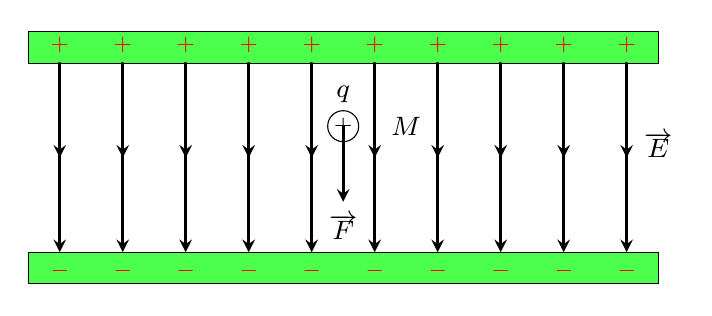
\begin{tikzpicture}[line join = round,line cap=round,>=stealth,font=\footnotesize,scale=0.8]
				 \draw[fill=green!70]
					(-0.5,0) rectangle  (9.5,0.5)
					(-0.5,-3)  rectangle (9.5,-3.5);
				\foreach \x  in {0,1,2,3,4,5,6,7,8,9}{
					\draw[->,line width=1pt] (\x,0) node[above,red]{$+$} --(\x,-1.5); 
					 \draw[->,line width=1pt] (\x,0) --(\x,-3) node[below,red]{$-$};
				} 
				\draw[->,line width=1pt]  (4.5,-1)--(4.5,-2.2) node[below,scale=1.2]{$\overrightarrow{F}$};
				\draw 
					(4.5,-0.5) node[scale=1.2]{$q$} 
					(4.5,-1) circle (7pt) node[scale=1]{$+$} 
					 (5.5,-1) node[scale=1.2]{$M$}
					(9.5,-1.3) node[scale=1.2]{$\overrightarrow{E}$}; 
			\end{tikzpicture}
	\end{center}
	\loigiai{ 
		Độ  lớn của lực tĩnh điện tác dụng lên điện tích điểm là
		$$F = q\cdot E = 2  \cdot 10^{-9} \cdot 10^5 = 10^{-4}~ \mathrm{N}.$$
		 Suy ra $a+b=1-4=3$.
	 }
\end{bt}

% nguồn: Lop_12_Hinh_hoc_Chuong_2
\begin{bt}%[ma:64295083]
	%[2H2V2-2] 
	Một máy bay đang  cất cánh từ phi trường với tọa độ $M(a;b;c)$ trong đó $a$, $b$ và $c$ khác $0$. Với hệ toạ độ không gian $Oxyz$ được thiết lập như hình vẽ, cho biết $M$ là vị trí của máy bay, $OM=14$, $\widehat{NOB}=32^{\circ}$, $\widehat{MOC}=65^{\circ}$. Biết điểm $M(a;b;c)$. Tính tổng $a+2b+3c$ (kết quả làm tròn kết quả đến hàng đơn vị)
	 \shortans{39}
	\loigiai{ 
		 Gọi các điểm $A$, $B$, $C$ lần lượt là hình chiếu của điểm $M$ lên trục $Ox$, $Oy$, $Oz$.\\
		Điểm $N$ là hình chiếu của điểm $M$ lên $(Oxy)$.\\ 
		Ta có $\triangle COM$ vuông ở $C\Rightarrow  OC=OM\cdot \cos65^{\circ}\approx5{,}92\Rightarrow c\approx5{,}92$.\\
		Do  đó $CM=OM\cdot \sin65^{\circ}\approx12{,}69\Rightarrow ON=CM\approx12{,}69$.\\
		Ta có $\triangle BON$ vuông ở $B\Rightarrow  OB=ON\cdot \cos32^{\circ}\approx10{,}76\Rightarrow b\approx10{,}76$.\\
		 Suy ra $BN=ON\cdot \sin32^{\circ}\approx6{,}72\Rightarrow OA=BN\approx6{,}72\Rightarrow a\approx6{,}72$.\\
		Do đó $M(6{,}72;10{,}76;5{,}92)\Rightarrow  a+2b+3c\approx39{,}27\approx39$.
	} 
\end{bt}

% nguồn: Lop_12_Hinh_hoc_Chuong_2
\begin{bt}%[ma:75944ec6]
	%[2H2V1-4] 
	Cho hình lập phương $ABCD.A'B'C'D'$. Gọi $M$, $N$ lần lượt~là trung điểm của $A'D$ và $C'D'$. Gọi $\varphi$~là góc giữa hai vectơ $\overrightarrow{MN}$ và $\vec{A'B}$. Số đo  của góc $\varphi$ bằng bao nhiêu độ? \shortans{90}
	 \loigiai{
	\immini{ 
		Trong không gian  $Oxyz$, chọn\\
		$\begin{aligned}
		O\equiv& A(0;0;0)  \Rightarrow A'(0;0;a)\\
		& B(a;0;0) \Rightarrow  B'(a;0;a)\\
		& C(a;a;0) \Rightarrow C'(a;a;a)\\ 
		& D(0;a;0) \Rightarrow D'(0;a;a).\\ 
	\end{aligned}$\\
	Điểm $M$~là trung điểm  của $A'D \Rightarrow M\left(0;\dfrac{a}{2};\dfrac{a}{2}\right)$;\\
	Điểm $N$~là trung điểm của $C'D'  \Rightarrow N\left(\dfrac{a}{2};a;a\right)$.\\
	 Suy ra
	\begin{align*}
		 & \overrightarrow{MN}=\left(\dfrac{a}{2};\dfrac{a}{2};\dfrac{a}{2}\right)\\
		& \vec{A'B}=\left(a;0;-a\right)\\ 
		& \overrightarrow{MN}\cdot\vec{A'B}=\dfrac{a}{2}\cdot a +  \dfrac{a}{2}\cdot 0 + \dfrac{a}{2}\cdot(-a) =0.
	\end{align*}
	 Suy ra $\overrightarrow{MN}\perp\vec{A'B}$.
	Vậy  $\varphi = 90^\circ$.
	 }
	{\resizebox{!}{5cm}{\begin{tikzpicture}[line cap=round,line join=round]
		 \def\a{3}
		\path (0:0)  coordinate (A)
			(0:\a) coordinate (D) 
			($(D)+(0:10mm)$)  coordinate (y)
			 (240:\a/1.5) coordinate (B)
			($(B)+(240:10mm)$)  coordinate (x)
			($(B)+(D)-(A)$)  coordinate (C)
			($(A)+(90:\a)$) coordinate  (A')
			($(A')+(90:10mm)$) coordinate  (z)
			($(B)+(90:\a)$) coordinate  (B')
			($(C)+(90:\a)$) coordinate (C') 
			($(D)+(90:\a)$)  coordinate (D')
			 ($(A')!1/2!(D)$) coordinate (M)
			($(C')!1/2!(D')$) coordinate  (N);
		 \draw[dashed] (B)--(A)--(D)
			(A)--(A')--(D); 
		\draw  (A')--(B')--(C')--(D')--cycle (B')--(B)--(C)--(D)--(D')
			(C)--(C'); 
		 \draw[teal,-stealth,dashed] (M)--(N);
		\draw[teal,-stealth,dashed]  (A')--(B);
		\foreach \x/\pos in {A/160,B/180,C/0,D/45,A'/160,B'/180,C'/0,D'/90,M/180,N/90,x/160,y/90,z/180}  \fill (\x) circle (1pt) node[{shift=(\pos:10pt)}]{$\x$};
		\foreach \x/\y  in {B/x,D/y,A'/z}{\draw[-stealth] (\x)--(\y);}
	\end{tikzpicture}
	} 
}} 
\end{bt}

% nguồn: Lop_12_Hinh_hoc_Chuong_2
\begin{bt}%[ma:37028b1d]
	%[2H2C2-2] 
	\immini{ 
	Một bể cá dạng hình hộp chữ nhật $ABCD. EFGH$ với $AB = 6$dm, $AD = 8$dm và $AE = 8$dm. Một chú cá con bơi theo những đoạn thẳng từ điểm $G$ đến chạm mặt đáy của hồ, rồi từ điểm đó bơi đến vị trí điểm $M$ là trung điểm của $AF$. Để đường đi ngắn nhất thì chú cá bơi đến điểm dưới đáy hồ cách $BA$ và $BC$ những đoạn bằng $a$ và $b$. Khi đó tổng $D = 3a + 6b$ bằng bao~nhiêu? 
	 }{
	\begin{tikzpicture}[>=stealth,line join = round,line cap = round]
			\clip  (-0.5,-3.5) rectangle (6,2.5);
			 \coordinate (A) at (0,0);
			\coordinate (B) at  (2,0);
			 \coordinate (D) at (3.5,-2.5);
			 \coordinate (C) at ($(B)+(D)-(A)$);
			\coordinate  (E) at ($(A)+(0,2)$);
			 \coordinate (F) at ($(B)+(E)-(A)$);
			\coordinate (H) at  ($(E)+(D)-(A)$);
			\coordinate (G) at ($(C)+(E)-(A)$); 
			 \coordinate (M) at ($(A)!0.5!(F)$);
			 \draw (E)--(A)--(D)--(C)--(G)--(F)--(E)--(H)--(G)
				 (H)--(D);
			\draw[dashed]  (B)--(F)--(A)--(B)--(C);
			\foreach \x/\g in{A/180,B/-90,C/-30,D/-120,M/150,E/120,F/60,H/60,G/60}\fill (\x) circle  (1pt) node[shift={(\g:10pt)}]{$\x$};
		\end{tikzpicture}
	 }
	\shortans{20} 
	 \loigiai{
	 \immini{
		 Gắn hình vẽ vào hệ trục tọa độ $Oxyz$ vuông góc, mỗi đơn vị trên hệ trục bằng $1$dm, sao cho $A$ trùng với $O$; $D$, $B$, $E$ lần lượt thuộc các trục $Ox$, $Oy$, $Oz$ như hình vẽ.\\
		Khi đó ta có mặt  đáy của bể nằm trên mặt phẳng $(Oxy)$ và $A(0;0;0)$, $F(0;6;10)$, $G(8;6;10)$.\\
		Vì $M$ là trung  điểm $AF$ nên $M$ có tọa độ $M(0;3;5)$.\\
		Gọi $G'$ là điểm  đối xứng của $G$ qua $(Oxy)$ thì $G'(8;6;-10)$.\\
		Gọi $I(x;y;0)$ là điểm mà con cá chạm mặt đáy bể, khi đó 
		$$MI+IG=MI+IG'\ge  MG'.$$}{
		\begin{tikzpicture}[>=stealth,line join = round,line cap = round]
				\clip (-0.5,-5.5) rectangle (6,3.5); 
				\coordinate (A) at  (0,0);
				\coordinate (B)  at (2,0);
				\coordinate  (D) at (3.5,-2);
				 \coordinate (C) at ($(B)+(D)-(A)$);
				\coordinate (E) at ($(A)+(0,2)$); 
				\coordinate (F) at  ($(B)+(E)-(A)$);
				\coordinate  (H) at ($(E)+(D)-(A)$);
				\coordinate  (G) at ($(C)+(E)-(A)$);
				\coordinate  (G') at ($(C)!-1!(G)$);
				 \coordinate (M) at ($(A)!0.5!(F)$);
				\coordinate (x')  at ($(A)!0.5!(B)$);
				\coordinate  (I) at ($(M)!1/3!(G')$);
				\coordinate (z') at  ($(M)!0.62!(G')$);
				\draw (E)--(A)--(D)--(C)--(G)--(F)--(E)--(H)--(G) 
					 (H)--(D)
					(C)--(G')--(z'); 
				\draw[dashed]  (B)--(F)--(A)--(B)--(C)
					(M)--(z') 
					(I)--(G); 
				 \coordinate (x) at ($(A)!1.2!(D)$);
				\draw[->] (D)--(x) node[above]{$x$}; 
				\coordinate (y) at  ($(A)!1.5!(B)$);
				\draw[->,dashed] (B)--(y) node[below]{$y$}; 
				\coordinate  (z) at ($(A)!1.4!(E)$);
				\draw[->]  (E)--(z) node[right]{$z$};
				\foreach \x/\g in{A/180,B/30,C/-30,D/-120,M/150,E/180,F/60,H/60,G/60,I/180,G'/-90}\fill (\x) circle  (1pt) node[shift={(\g:10pt)}]{$\x$};
			\end{tikzpicture}
		} 
		Đẳng thức xảy ra  khi $M$, $I$, $G$ thẳng hàng, tức là $\overrightarrow{MI}=k\overrightarrow{MG'}$. \\
		Ta  có
		$$\heva{& x=8k  \\ & y-3=3k\\ & -5=-15k}\Leftrightarrow\heva{& x=\dfrac{8}{3} \\ & y=4\\ & k=\dfrac{1}{3}.}$$
		Vậy quãng đường ngắn nhất khi $I$ có tọa  độ $I\left(\dfrac{8}{3};4;0\right)$.\\
		Khoảng cách từ $I$  đến $AB$ là $a=x_I=\dfrac{8}{3}$.\\
		Khoảng cách từ $I$ đến $BC$  là $b=6-y_I=2$.\\
		Vậy  $3a+6b=8+12=20$.
	 }
\end{bt}

% nguồn: Lop_12_Hinh_hoc_Chuong_2
\begin{bt}%[ma:8bc72f49]
	%[2H2V2-2] 
	Trong không gian với hệ tọa độ $Oxyz$, cho hai điềm $A(1;2;3)$, $B(7;10;6)$. Hai điểm $M$, $N$ thay đổi trên mặt phẳng $(Oxy)$ sao cho $MN=4$. Khi $AM+BN$ nhỏ nhất, tính tổng hoành  độ của $M$ và tung độ của $N$.
	 \shortans{9}
	 \loigiai{
		\begin{center}
			\resizebox{!}{5cm}{ 
			\begin{tikzpicture}[line join = round,line cap=round,>=stealth]
					 \path
						(-3,-1) coordinate (x) 
						(-1,2) coordinate (y) 
						 (6,2) coordinate (z)
						 (4,-1) coordinate (t)
						(0,4) coordinate  (A)
						(0,1) coordinate  (C)
						(4,5) coordinate (B) 
						 (4,1) coordinate (D)
						 (0.5,0) coordinate (M)
						(3,0.2) coordinate (N); 
					\draw (x)--(y)--(z)--(t)--cycle (A)--(C) 
						 (C)--(M)--(N)--(D)--cycle (B)--(D)
						(A)--(M) 
						 (B)--(N);
					\foreach  \p/\pos in {A/90,B/90,C/180,D/0,M/-90,N/-90}
					\fill (\p) circle (1pt)  node[shift={(\pos:3mm)}] {$\p$};
					\draw pic["$(Oxy)$"rotate=20,angle eccentricity=.6,angle radius=1.5cm] 
						{angle=t--x--y}; 
				\end{tikzpicture}
			} 
		\end{center}
		Gọi $C$, $D$ lần lượt là hình chiếu vuông góc của $A$, $B$ trên  mặt phẳng $(Oxy)$.\\
		Suy ra tọa  độ $C(1;2;0)$, $D(7;10;0)$.\\
		 Khi đó $CD=\sqrt{(7-1)^2+(10-2)^2+0^2}=10$.\\
		 Ta có $AM+BN=\sqrt{AC^2+CM^2}+\sqrt{BD^2+DN^2}=\sqrt{9+CM^2}+\sqrt{36+DN^2}$.\\
		Khi đó $AM+BN$ nhỏ  nhất khi $C$, $M$, $N$, $D$ thẳng hàng.\\
		Đặt $CM=x$ với $0<x<6$. Suy ra $ND=6-x$.\\ 
		 Ta có $AM+BN=\sqrt{9+x^2}+\sqrt{36+(6-x)^2}=\sqrt{9+x^2}+\sqrt{x^2-12x+72}$.\\
		 Xét hàm số $f(x)=\sqrt{9+x^2}+\sqrt{x^2-12x+72}$ với $0<x<6$.\\
		Ta có  $f’(x)=\dfrac{x}{\sqrt{9+x^2}}+\dfrac{x-6}{\sqrt{x^2-12x+72}}$.\\
		Khi đó  $f’(x)=0\Leftrightarrow\dfrac{x}{\sqrt{9+x^2}}+\dfrac{x-6}{\sqrt{x^2-12x+72}}=0\Leftrightarrow x=2$.\\
		Bảng biến thiên 
		\begin{center}
			
\begin{tikzpicture}
					 \tkzTabInit[nocadre,lgt=1.2,espcl=2.5,deltacl=0.7]
						{$x$ /.6,$f'(x)$ /0.6,$f (x)$  /2}
						{$0$,$2$,$6$} 
					 \tkzTabLine{,-,$0$,+,}
					 \tkzTabVar{+/,-/$3\sqrt{13}$,+/}
				\end{tikzpicture}
		\end{center}
		Vậy $\min(AM+BN)=3\sqrt{13}$ khi $CM=x=2$.\\ 
		Khi đó $\overrightarrow{CM}=\dfrac{1}{5}\overrightarrow{CD}$. Suy ra $x_M=x_C+\dfrac{1}{5}(x_D-x_C)=\dfrac{11}{5}$.\\ 
		Mặt khác  $\overrightarrow{CN}=\dfrac{3}{5}\overrightarrow{CD}$. Suy ra $y_N=y_C+\dfrac{3}{5}(y_D-y_C)=\dfrac{34}{5}$.\\
		Vậy tổng hoành độ của $M$ và tung độ của $N$  là $x_M+y_N=\dfrac{11}{5}+\dfrac{34}{5}=9$.
	 }
\end{bt}

% nguồn: Lop_12_Hinh_hoc_Chuong_2
\begin{bt}%[ma:709ddb7d]
	%[2H2V1-4] 
	Cho hình lập phương $ABCD.A'B'C'D'$ có cạnh bằng $a$. Gọi $M$, $N$ lần lượt~là trung điểm của $A'D'$ và $C'D'$. Tích vô  hướng $\overrightarrow{MN}\cdot\vec{C'B}=na^2$ ($n$~là số thập phân). Giá trị của $n$ bằng bao nhiêu?
	\shortans{-0,5} 
	\loigiai{ 
	\immini{ 
		Trong không gian $Oxyz$, chọn\\ 
		$\begin{aligned}
		O\equiv& A(0;0;0)  \Rightarrow A'(0;0;a)\\
		& B(a;0;0) \Rightarrow  B'(a;0;a)\\
		& C(a;a;0)  \Rightarrow C'(a;a;a)\\
		 & D(0;a;0) \Rightarrow D'(0;a;a).\\
	\end{aligned}$\\
	Điểm $M$~là trung điểm của $A'D'  \Rightarrow M\left(0;\dfrac{a}{2};a\right)$;\\
	Điểm $N$~là  trung điểm của $C'D' \Rightarrow N\left(\dfrac{a}{2};a;a\right)$.\\
	Suy  ra
	$\begin{aligned}
	& \overrightarrow{MN}=\left(\dfrac{a}{2};\dfrac{a}{2};0\right)\\ 
	&  \vec{C'B}=\left(0;-a;-a\right)\\
	&  \overrightarrow{MN}\cdot\vec{C'B}=\dfrac{a}{2}\cdot0+\dfrac{a}{2}\cdot(-a)+0\cdot(-a)=-\dfrac{1}{2}a^2.
	\end{aligned}$\\
	Vậy $n=-\dfrac{1}{2}=-0{,}5$. 
	 }{
	\begin{tikzpicture}[line cap=round,line join=round]
			\def\a{3} 
			\path (0:0) coordinate (A) 
				 (0:\a) coordinate (D)
				($(D)+(0:10mm)$) coordinate (y) 
				 (240:\a/1.5) coordinate (B)
				 ($(B)+(240:10mm)$) coordinate (x)
				($(B)+(D)-(A)$)  coordinate (C)
				($(A)+(90:\a)$) coordinate  (A')
				($(A')+(90:10mm)$) coordinate  (z)
				($(B)+(90:\a)$) coordinate (B') 
				($(C)+(90:\a)$)  coordinate (C')
				($(D)+(90:\a)$) coordinate (D') 
				($(A')!1/2!(D')$) coordinate  (M)
				 ($(C')!1/2!(D')$) coordinate (N)
				($(A)!1/2!(B)$)  coordinate (P);
			\draw[dashed,thin]  (B)--(A)--(D)
				 (A)--(A');
			\draw (A')--(B')--(C')--(D')--cycle  (B')--(B)--(C)--(D)--(D')
				(C)--(C'); 
			 \draw[teal,-stealth] (M)--(N);
			\draw[teal,-stealth]  (C')--(B);
			\draw[teal,-stealth,dashed]  (M)--(P)
				 (N)--(P);
			\foreach \x/\y in {A/160,B/180,C/0,D/45,A'/160,B'/180,C'/0,D'/90,M/90,N/0,P/180,x/160,y/90,z/180} 
			\fill (\x) circle  (1pt) node[shift={(\y:10pt)}] {$\x$};
			\foreach  \x/\y in {B/x,D/y,A'/z}{\draw[-stealth] (\x)--(\y);}
		\end{tikzpicture}
	} 
} 
\end{bt}

% nguồn: Lop_12_Hinh_hoc_Chuong_2
\begin{bt}%[ma:985009ab]
	%[2H2V2-6] 
	Trượt nước là một trong những trò chơi vận động được nhiều người yêu thích trong các công viên nước. Một cái máng trượt nước có thiết kế dạng cung tròn với hai đầu mút là $A$ và $B$. Chọn một trục tọa độ $Oxyz$ với gốc $O$ đặt tại hình chiếu của điểm $A$ trên mặt  đất, mặt phẳng $(Oxy)$ trùng với mặt đất và trục $Oz$ hướng thẳng đứng lên trên trời, đơn vị đo lấy theo mét (tham khảo hình vẽ dưới đây). Biết các điểm $A,B$ và một điểm $C$ nằm trên máng trượt lần lượt có toạ độ là $(0;0;5);(6;7;1)$ và $(5;0;2)$. Độ dài máng trượt nước đó bằng bao~nhiêu mét (làm tròn kết quả đến hàng đơn vị của mét)?
	\shortans{14} 
	 \loigiai{
		Ta có  $A(0;0;5)$, $B(6;7;1)$, $C(5;0;2)$.
		Suy ra $\overrightarrow{AB}=(6;7;-4)$ và $\overrightarrow{AC}=(5;0;-3)$.\\ 
		Phương trình mặt phẳng $(ABC)$ đi qua $A(0;0;5)$ và có  véc-tơ pháp tuyến
		\[\vec{n}=[\overrightarrow{AB},\overrightarrow{AC}]=(21;2;35)\]  có phương trình là $21x+2y+35z-175=0$.\\
		Mặt phẳng trung trực $(\alpha)$ của đoạn $AB$ đi  qua $M\left(3;\dfrac{7}{2};3\right)$ có vectơ pháp tuyến $\overrightarrow{AB}=(6;7;-4)$.\\
		 Do đó $(\alpha)$ có phương trình là $6x+7y-4z-\dfrac{61}{2}=0$.
		Mặt phẳng trung trực của đoạn $AC$ đi qua  $N\left(\dfrac{5}{2};0;\dfrac{7}{2}\right)$ có vectơ pháp tuyến $\overrightarrow{AC}=(5;0;-3)$ có phương trình là $5x-3z-2=0$.\\
		Gọi $I$ là tâm đường tròn ngoại tiếp tam giác $ABC$. Toạ độ điểm $I$ là nghiệm của hệ phương  trình
		\[\heva{&{21x+2y+35z-175=0}\\ 
		 &{6x+7y-4z-\dfrac{61}{2}=0}\\
		&{5x-3z-2=0} 
		 }\Leftrightarrow\heva{&x=\dfrac{1999}{835}\\
		&y=\dfrac{7021}{1670}\\ 
		 &z=\dfrac{555}{167}.
		 }\]
		Từ đây tính  được $R=IA=\sqrt{\left(-\dfrac{1999}{835}\right)^2+\left(-\dfrac{7021}{1670}\right)^2+\left(5-\dfrac{555}{167}\right)^2}\approx5{,}1203$ mét.\\
		Gọi $\varphi$ là là góc giữa hai  vectơ $\overrightarrow{IA}$ và $\overrightarrow{IB}$ ta tính được
		\[\overrightarrow{IA}=\left(-\dfrac{1999}{835};-\dfrac{7021}{1670};\dfrac{280}{167}\right);\,\overrightarrow{IB}=\left(\dfrac{3011}{835};\dfrac{4669}{1670};-\dfrac{388}{167}\right);\,\cos\varphi=\dfrac{\overrightarrow{IA}\cdot  \overrightarrow{IB}}{IA\cdot IB}\Rightarrow\varphi\approx2{,}754955.\]
		Độ dài máng trượt là là  độ dài cung $l_{AB}=R\varphi\approx14$ mét.
	 }
\end{bt}

% nguồn: Lop_12_Hinh_hoc_Chuong_2
\begin{bt}%[ma:1bfe5e17]
	%[2H2H1-1] 
	Cho hình hộp $ABCD. A_1 B_1 C_1 D_1$. Tìm giá trị của thích hợp điền vào đẳng thức véc  tơ $\overrightarrow{AB}+\overrightarrow{B_1 C_1}+\overrightarrow{DD_1}=k\overrightarrow{AC_1}$.
	\shortans{1} 
	 \loigiai{
	\immini{Ta có $\overrightarrow{AB}+\overrightarrow{B_1 C_1}+\overrightarrow{DD_1}=\overrightarrow{AB}+\overrightarrow{AD}+AA_1=\overrightarrow{AC_1}$.  Suy ra $k=1$.}{
		\begin{tikzpicture}[declare function={a=5; b=0.45*a; h=0.65*a;}]
				\path (0:0)  coordinate (A)
					(220:b) coordinate  (B)
					 ($(B)+(a,0)$) coordinate (C)
					(a,0) coordinate (D) 
				\foreach  \x in {A,B,C,D}{(\x)++(90:h) coordinate (\x1)};
				\draw[dashed]  (A)--(B)
					 (A)--(D);
				\draw[->,dashed]  (A1)--(A)
					 (B1)--(D);
				 \draw[->] (B1)--(D1);
				 \draw (B1)--(A1)--(D1)--(C1)
					(D1)--(D)--(C) 
					 (B)--(C)--(C1)--(B1)--cycle;
				\foreach \x/\goc/\t in  {A/180/D_1,B/-90/A_1,C/-90/B_1,D/0/C_1,A1/180/D,B1/180/A,C1/0/B,D1/90/C}
				\fill (\x) circle  (1pt) node[shift={(\goc:7pt)},font=\scriptsize]{$\t$};
			\end{tikzpicture}
		} 
	 }
\end{bt}

% nguồn: Lop_12_Hinh_hoc_Chuong_2
\begin{bt}%[ma:f2212098]
	 %[2H2H1-1]
	Trong không gian $Oxyz$, cho hai đường thẳng $\Delta_{1}\colon \dfrac{x+24}{3}=\dfrac{y-25}{4}=\dfrac{z}{-5}$ và $\Delta_{2}\colon\dfrac{x-26}{5}=\dfrac{y}{3}=\dfrac{z}{4}$. Góc giữa hai đường thẳng  $\Delta_{1}$, $\Delta_{2}$ bằng bao nhiêu độ (làm tròn đến hàng đơn~vị của~độ)?\shortans{82}
	 \loigiai{
		Theo lí thuyết. Cho hai  đường thẳng $\Delta_1$ và $\Delta_2$ có vectơ chỉ phương lần lượt~là $\overrightarrow{u_1}=\left(a_1;b_1;c_1\right)$, $\overrightarrow{u_2}=\left(a_2;b_2;c_2\right)$.\\
		Khi đó, ta có $\cos\left(\Delta_1,\Delta_2\right) = \dfrac{\vert  a_{1}a_{2}+b_{1}b_{2}+c_{1}c_{2} \vert}{\sqrt{a_{1}^2+b_{1}^2+c_{1}^2}\cdot \sqrt{a_{2}^2+b_{2}^2+c_{2}^2}}$.\\
		Theo bài, ta có $\Delta_1$ có vectơ chỉ phương~là $\overrightarrow{u_1}=\left(3;4;-5\right)$, $\Delta_2$ có  vectơ chỉ phương~là $\overrightarrow{u_2}=\left(5;3;4\right)$.\\
		Khi đó $\cos\left(\Delta_1,\Delta_2\right)  = \dfrac{\left|3\cdot 5+4\cdot 3+\left(-5\right)\cdot 4\right|}{\sqrt{3^2+4^2+\left(-5\right)^2}\cdot \sqrt{5^2+3^2+4^2}}=\dfrac{7}{50}$.\\
		Tìm được  góc $\left(\Delta_1,\Delta_2\right)\approx 82^{\circ}$.
	 }
\end{bt}

% nguồn: Lop_12_Hinh_hoc_Chuong_2
\begin{bt}%[ma:83a769a2]
	 %[2H2V2-4]
	Cho hàm số $ y=f(x)=\dfrac{2x^2+26x+18}{x+13}$ có điểm cực  tiểu $ x=x_1$ và điểm cực đại $x=x_2$. Tính $P=-2x_1+x_2$.
	 \shortans{4}
	 \loigiai{
		Ta có 
		$ y'=f'(x)=\dfrac{(4x+26)(x+13)-(2x^2+26x+18)}{(x+13)^2}=\dfrac{2x^2+52x+320}{(x+13)^2}$.\\ Suy ra $ y'=0\Leftrightarrow 2x^2+52x+320=0 \Leftrightarrow\hoac{& x=-16\\ &  x=-10.}$\\
		Hàm số đạt cực  tiểu tại $ x=x_1=-10$ và đạt cực đại tại $ x=x_2=-16$.\\
	Khi đó $P=-2x_1+x_2=-2(-10)-16=4$.} 
\end{bt}

% nguồn: Lop_12_Hinh_hoc_Chuong_2
\begin{bt}%[ma:90ce2e5a]
	 %[2H2V2-2]
	Trong không gian $Oxyz$, cho các điểm $A(1;-1;2)$, $B(-1;1;1)$, $C(-3;-3;4)$,  $D\left(1;\dfrac{1}{2};1\right)$. Điểm $M$ thay đổi trên mặt phẳng $(Oxy)$. Khi biểu thức $T=-3\left(\dfrac{MA}{MD}\right)^2-2\left(\dfrac{MB}{MD}\right)^2+\left(\dfrac{MC}{MD}\right)^2$ đạt giá trị lớn nhất thì hoành độ của điểm $M$ bằng bao~nhiêu?
	\shortans{1} 
	 \loigiai{
		Giả  sử $M(x;y;0)$.\\
		Ta  có
		\begin{itemize}
			\item $MA^2=(x-1)^2+(y-1)^2+4$. 
			\item  $MB^2=(x+1)^2+(y-1)^2+1$.
			\item  $MC^2=(x+3)^2+(y+3)^2+16$.
			\item $MD^2=(x-1)^2+\left(y-\dfrac{1}{2}\right)^2+1$. 
		\end{itemize}
		\begin{eqnarray*}
			 T&=&\dfrac{-3MA^2-2MB^2+MC^2}{MD^2}\\
			 &=&\dfrac{-4x^2+8x-4y^2+4y+10}{(x-1)^2+\left(y-\dfrac{1}{2}\right)^2+1}\\
			 &=&-4\cdot\dfrac{(x-1)^2+\left(y-\dfrac{1}{2}\right)^2+1-\dfrac{19}{4}}{(x-1)^2+\left(y-\dfrac{1}{2}\right)^2+1}\\
			&=&-4\cdot1+\dfrac{19}{(x-1)^2+\left(y-\dfrac{1}{2}\right)^2+1}\\ 
			 &\leq&-4+19\\
			 &=&15.
		\end{eqnarray*}
		Dấu bằng xảy ra khi và chỉ khi $\heva{&x=1\\&y=\dfrac{1}{2}}\Rightarrow  M\left(1;\dfrac{1}{2};0\right)$.\\
		Vậy biểu  thức $T$ đạt giá trị lớn nhất thì hoành độ điểm $M$ bằng $1$.
	} 
\end{bt}

% nguồn: Lop_12_Hinh_hoc_Chuong_2
\begin{bt}%[ma:6ae8afbd]
	 %[2H2H1-4]
	Một chiếc máy đo đạc trắc địa được đặt trên một giá đỡ ba chân. Trọng lực tác dụng lên chiếc máy có độ lớn là $30$ N và được phân bố thành ba lực $\overrightarrow{F_1}$, $\overrightarrow{F_2}$, $\overrightarrow{F_3}$ lên ba chân của giá đỡ. Ba lực $\overrightarrow{F_1}$, $\overrightarrow{F_2}$, $\overrightarrow{F_3}$ có độ lớn bằng nhau và góc tạo bởi mỗi chân của giá đỡ và mặt đất là $60^{\circ}$. Hỏi độ lớn của lực $\overrightarrow{F_1}$ là bao~nhiêu N  (làm tròn kết quả đến hàng phần chục)?
	 \shortans{11,5}
	\loigiai{ 
		\begin{center}
			\resizebox{!}{5cm}{\begin{tikzpicture}[line join = round,line cap=round,>=stealth]
		\coordinate (A) at (-2,0); 
		\coordinate (B) at  (-2,-2);
		\coordinate  (C) at (5,0);
		\coordinate (M) at  ($(A)!0.5!(B)$);
		\coordinate (H) at  ($(C)!2/3!(M)$);
		\coordinate  (S) at ($(H)+(0,5)$);
		\coordinate (E) at ($(S)!.4!(A)$); 
		\coordinate (F)  at ($(S)!.3!(B)$);
		\coordinate (G) at ($(S)!.4!(C)$); 
		\pic[draw,thin,angle radius=1.5mm] {right angle =  A--H--S};
		\draw  (S)--(A)
			 (S)--(B)
			(S)--(C) 
			 (B)--(C)
			 (A)--(B);
		 \draw[dashed](A)--(C)
			(A)--(H) 
			(S)--(H); 
		\draw[orange,->] (S)--(E); 
		\draw[orange,->]  (S)--(F);
		\draw[orange,->]  (S)--(G);
		\node[above]  at (-1.2,2.1) {$\overrightarrow{F_1}$};
		\node[above]  at (-.56,1.7) {$\overrightarrow{F_2}$};
		\node[above] at  (1.5,2.1) {$\overrightarrow{F_3}$};
		\foreach \p/\pos in {S/90,A/180,B/-90,C/0,H/-70} 
		\fill (\p) circle (1pt) node[shift={(\pos:3mm)}] {\p}; 
	\end{tikzpicture}
			 }
		\end{center}
		Giả sử chiếc máy đo đạc được đặt ở điểm $S$; mặt phẳng $(ABC)$ là mặt đất; ba chân của giá đỡ  tương ứng với ba cạnh $SA$, $SB$, $SC$; các lực $\overrightarrow{F_1}$, $\overrightarrow{F_2}$, $\overrightarrow{F_3}$ được mô tả như hình vẽ.\\
		Gọi $H$ là trọng tâm của  tam giác $ABC$.\\
		Khi  đó, $SH\perp(ABC)$ và $\overrightarrow{HA}+\overrightarrow{HB}+\overrightarrow{HC}=\overrightarrow{0}$.\\
		Vì ba lực $\overrightarrow{F_1},\overrightarrow{F_2},\overrightarrow{F_3}$ có độ lớn bằng nhau và góc tạo bởi mỗi chân của giá đỡ và mặt đất là $60^{\circ}$ nên tồn tại số  thực $k(k\neq 0)$ để $\overrightarrow{F_1}=k\overrightarrow{SA}$, $\overrightarrow{F_2}=k\overrightarrow{SB}$, $\overrightarrow{F_3}=k\overrightarrow{SC}$ và $\widehat{SAH}=60^{\circ}$.\\
		Ta có $\overrightarrow{F_1}+\overrightarrow{F_2}+\overrightarrow{F_3}=k\left(\overrightarrow{SA}+\overrightarrow{SB}+\overrightarrow{SC}\right)=k\left(3\overrightarrow{SH}+\overrightarrow{HA}+\overrightarrow{HB}+\overrightarrow{HC}\right)=3k\overrightarrow{SH}$.\\ 
		Lại có $\overrightarrow{F_1}+\overrightarrow{F_2}+\overrightarrow{F_3}=\overrightarrow{P}$, ở đó $\overrightarrow{P}$ là trọng lực tác dụng lên chiếc máy đo đạc và  $\left|\overrightarrow{P}\right|=30$N.\\
		Khi đó, $3k\overrightarrow{SH}=\overrightarrow{P}$. Suy ra $3k\left|\overrightarrow{SH}\right|=\left|\overrightarrow{P}\right|=30$, do đó $SH=\left|\overrightarrow{SH}\right|=\dfrac{30}{3k}=\dfrac{10}{k}$.\\ 
		Tam giác $SAH$ vuông tại $H$ nên $SA=\dfrac{SH}{\sin\widehat{SAH}}=\dfrac{\dfrac{10}{k}}{\sin  60^{\circ}}=\dfrac{20\sqrt{3}}{3k}$.\\
		Suy ra $\left|\overrightarrow{F_1}\right|=k\left|\overrightarrow{SA}\right|=\dfrac{20\sqrt{3}}{3}\approx 11{,}5$  (N).\\
	Vậy độ lớn của lực $\overrightarrow{F_1}$ xấp  xỉ bằng $11{,}5$ N.}
\end{bt}

% nguồn: Lop_12_Hinh_hoc_Chuong_2
\begin{bt}%[ma:b9234f62]
	 %[2H2V1-2]
	Cho tứ diện $SABC$ có $G$ là trọng  tâm tam giác $ABC$ và $I$ là trọng tâm tam giác $GBC$. Biết $\overrightarrow{SI}=x\overrightarrow{SA}+y\overrightarrow{SB}+z\overrightarrow{SC}$, tính giá trị biểu thức $9\left(x-y+z\right)$.
	 \shortans{1}
	 \loigiai{
		Do $I$ là trọng tâm tam giác $GBC$ nên ta có: $\overrightarrow{SI}=\dfrac{1}{3} \left(\overrightarrow{SG}+\overrightarrow{SB}+\overrightarrow{SC}\right) (1)$.  \\
		Do $G$ là trọng tâm tam giác $ABC$  nên ta có: $$\overrightarrow{SG}=\dfrac{1}{3} \left(\overrightarrow{SA}+\overrightarrow{SB}+\overrightarrow{SC}\right) (2)$$
		Thay $(2)$ vào $(1)$ ta có: $\overrightarrow{SI}=\dfrac{1}{3} \left[\dfrac{1}{3} \left(\overrightarrow{SA}+\overrightarrow{SB}+\overrightarrow{SC}\right)+\overrightarrow{SB}+\overrightarrow{SC}\right]=\dfrac{1}{9} \overrightarrow{SA}+\dfrac{4}{9} \overrightarrow{SB}+\dfrac{4}{9} \overrightarrow{SC}$. \\ 
		Vậy $\heva{&{x=\dfrac{1}{9}} \\ &{y=\dfrac{4}{9}}  \\ &{z=\dfrac{4}{9}}} \Rightarrow 9(x-y+z)=1$.
	} 
\end{bt}

% nguồn: Lop_12_Hinh_hoc_Chuong_2
\begin{bt}%[ma:e82f6d50]
	%[2H2V2-6] 
	Có hai trạm thu phát sóng tín hiệu mặt đất đặt ở hai điểm $O$, $A$ và vệ tinh thu phát tín hiệu tại ở vị trí $M$, biết vệ tinh di chuyển luôn cách mặt đất $35\;000$ km. Tín hiệu tại $O$ phát lên vệ tinh $M$ rồi truyền đến trạm thu tại $A$. Xét hệ trục $Oxyz$ được chọn thỏa $O(0;0;0)$, $A(30; 40; 0)$, $M(x;y;35)$ (đơn vị tọa độ là ngàn km). Biết vận tốc  trung bình truyền tín hiệu giữa vệ tinh với trạm thu phát khoảng $270\;000$ km/s. Một tín hiệu phát từ $O$ đến $M$, rồi truyền về $A$ mất ít nhất bao~nhiêu giây (làm tròn đến hàng phần trăm).
	\shortans{0,32} 
	 \loigiai{
		Vì điểm $M$ có tọa độ là $M(x;y;35)$ nên điểm $M$ luôn thuộc mặt phẳng $(P)\colon z=35$.\\ 
		Hai điểm $O(0;0;0)$, $A(30; 40; 0)$ nằm cùng phía đối với mặt phẳng  $(P)$.\\
		Gọi $O'$ đối xứng với $O$ qua mặt  phẳng $(P)$. Khi đó $O'(0;0;70)$.\\
		 Ta có
		\[T= OM+MA=O'M+MA\ge O'A=\sqrt{30^+40^2+70^2}=10\sqrt{74}.\] 
		Dấu bằng xảy ra khi và chỉ khi $O$, $M$, $A$ thẳng hàng.\\ 
		Thời gian ít nhất để $A$ nhận được tín  hiệu từ $O$ là $\dfrac{10\sqrt{74}}{270} \approx 0{,}32$ (s).
	 }
\end{bt}

% nguồn: Lop_12_Hinh_hoc_Chuong_2
\begin{bt}%[ma:1e4731e9]
	 %[2H2V2-6]
	Với hệ trục tọa độ $Oxyz$ sao cho $O$ nằm trên mặt nước, mặt phẳng $Oxy$ là mặt  nước, trục $Oz$ hướng lên trên (đơn vị đo: mét), một con chim bói cá đang ở vị trí cách mặt nước $2$ m, cách mặt phẳng $(Oxz)$, $(Oyz)$ lần lượt là $3$ m và $1$ m phóng thẳng xuống vị trí con cá, biết con cá cách mặt nước $50$ cm, cách mặt phẳng $(Oxz)$, $(Oyz)$ lần lượt là $1$ m và $1{,}5$ m. Tọa độ điểm $B$ lúc chim bói cá vừa tiếp xúc với mặt nước là $(a, b, c)$. Tính $T = 5a + 15b + 25c$.
	 \shortans{28}
	 \loigiai{
		Gọi $A$ là vị trí con cá, $C$ là vị trí con chim bói cá, điểm $B$ là điểm lúc chim bói cá vừa tiếp xúc với mặt nước  (xem hình vẽ dưới).
		\begin{itemize}
			\item Do chim bói cá cách mặt phẳng $(Oxz)$ và $(Oyz)$ lần lượt $3$ m và $1$ m, đồng thời cách mặt nước $2$ m nên điểm $C$ có toạ độ $(1;3;2)$. 
			\item Do con cá cách mặt phẳng $(Oxz)$ và $(Oyz)$ lần lượt $1$ m và $1{,}5$ m và cách  mặt nước $0{,}5$ m nên điểm $A$ có toạ độ $(1{,}5;1;-0{,}5)$.
			\item Khoảng cách từ  chim bói cá đến con cá là độ dài đoạn $AC$.
			\item  Ta có $\overrightarrow{AC}=(-0{,}5;2;2{,}5)$.
			Vì $B \in (Oxy)$ nên $B$  có toạ độ $\left(x_B;y_B;0\right)$.\\
			Ta  có $\vec{BC}=\left(1-x_B;3-y_B;2-0\right)=\left(1-x_B;3-y_B;2\right)$.\\
			Vì $A$, $B$, $C$ thẳng hàng  nên $\overrightarrow{AC}=k\vec{BC}$ hay $\heva{&k\left(1-x_B\right)=-0{,}5\\&k\left(3-y_B\right)=2\\&2k=2{,}5} \Leftrightarrow \heva{&k=\dfrac{5}{4}\\&x_B=\dfrac{7}{5}\\&y_B=\dfrac{7}{5}.}$\\
			Vậy $T = 5a + 15b + 25c = 5 \cdot 1{,}4 + 15 \cdot 1{,}4 +  25 \cdot 0 = 28$.
	\end{itemize}}
\end{bt}

% nguồn: Lop_12_Hinh_hoc_Chuong_2
\begin{bt}%[ma:9cd478ba]
	%[2H2V2-6] 
	Một chiếc máy quay phim có trọng lượng $300$ N được đặt trên một giá đỡ ba chân với điểm đặt $E(0;0;6)$ và các điểm tiếp xúc với mặt đất của ba chân lần lượt là  $A_1 (0;1;0)$, $A_2 \left(\dfrac{\sqrt{3}}{2};-\dfrac{1}{2};0\right)$, $A_3 \left(-\dfrac{\sqrt{3}}{2};-\dfrac{1}{2};0\right)$. Giả sử $\overrightarrow{F}_1 = (a;b;c)$ khi đó $a+3b-c$ bằng?
	 \shortans{150}
	 \loigiai{
		Ta có: $\overrightarrow{EA_1}=(0;1;-6)$; $\overrightarrow{EA_2}=\left(\dfrac{\sqrt{3}}{2};-\dfrac{1}{2};-6\right)$; $\overrightarrow{EA_3} = \left(-\dfrac{\sqrt{3}}{2};-\dfrac{1}{2};-6\right)$ \\ 
		$\Rightarrow EA_1=EA_2=EA_3=\sqrt{37}$. \\ $\left|\overrightarrow{F}_1 \right| = \left|\overrightarrow{F}_2 \right|=\left|\overrightarrow{F}_3\right|$ vì máy quay cân bằng và trọng lực của máy quay tác dụng đều  lên 3 chân của giá đỡ. Do đó: \\
		$\overrightarrow{F}_1 = k\overrightarrow{EA}_1=(0;k;-6k)$; $\overrightarrow{F}_2 = k \overrightarrow{EA}_2 = \left(\dfrac{\sqrt{3}}{2}  k;-\dfrac{1}{2} k;-6k\right)$ \\
		$\overrightarrow{F}_3 = k \overrightarrow{EA}_3 = \left(-\dfrac{\sqrt{3}}{2}  k;-\dfrac{1}{2} k;-6k\right)$ \\
		$\Rightarrow  \overrightarrow{F}_1+\overrightarrow{F}_2+\overrightarrow{F}_3=(0;0;-18k)$. \\
		Mà $\overrightarrow{F}_1+\overrightarrow{F}_2+\overrightarrow{F}_3=\vec{P}=(0;0;-300)\Rightarrow  -18k = 300 \Leftrightarrow k=\dfrac{50}{3}$. \\
		Vậy $\overrightarrow{F}_1 = \left(0;\dfrac{50}{3};-100\right)$. \\ 
		Suy ra $a+3b-c=150$. 
	} 
\end{bt}

% nguồn: Lop_12_Hinh_hoc_Chuong_2
\begin{bt}%[ma:97a6b6ff]
	 %[2H2V2-6]
	 Cho hình lăng trụ đứng $ABC. A'B'C'$ có tam giác $ABC$ vuông cân tại $A$, $AB=5$, $CC'=10$. Khoảng cách giữa hai đường thẳng $AC$ và $BC'$ bằng bao~nhiêu? (làm tròn kết quả đến hàng phần trăm).
	 \shortans{4,47}
	\loigiai{ 
		\begin{center}
			\begin{tikzpicture}[line join=round,line cap=round,font=\footnotesize,scale=1,>=stealth]
					\def  \r{2.5}
					 \path
						(0,0) coordinate (B) 
						 (60:0.7*\r) coordinate (A)
						(0:\r) coordinate (D) 
						 (-40:0.5*\r) coordinate (C)
						($(B)!0.5!(C)$) coordinate (M); 
					\draw[-stealth](A)--(B); 
					\draw[-stealth](A)--(C); 
					 \draw[-stealth](A)--(D);
					\draw  (B)--(C)--(D)
						(A)--(M); 
					 \draw[dashed] (B)--(D)
						 (M)--(D);
					\foreach \x/\g in {A/90,B/180,C/-90,D/0,M/-120}\fill (\x) circle  (1pt)+(\g:.3) node{$\x$};
				\end{tikzpicture}0
			 0
		\end{center}
		Chọn hệ trục tọa độ $Oxyz$ với $A$ trùng với gốc tọa độ $O$, cạnh $AB$ nằm trên trục $Ox$, cạnh $AC$ nằm trên trục $Oy$ và cạnh $AA'$ nằm  trên trục $Oz$. \\
		Khi đó  $A(0;0;0), B(5;0;0), C(0;5;0), A'(0;0;10)$. \\
		Vì $ACC'A'$ là hình bình hành nên $C'(0;5;10)$. \\ 
		Ta có $\overrightarrow{AC}=(0;5;0)$;  $\overrightarrow{BC'}=(-5;5;10)$; $[\overrightarrow{AC}, \overrightarrow{BC'}] = (50; 0; 25) \implies |[\overrightarrow{AC}, \overrightarrow{BC'}]| = 25\sqrt{5}$. \\
		Mặt khác $\overrightarrow{AB}=(5;0;0)$ nên $[\overrightarrow{AC}, \overrightarrow{BC'}]  \cdot \overrightarrow{AB} = 250$. \\
		Do đó, $d(AC, BC') = \dfrac{|[\overrightarrow{AC}, \overrightarrow{BC'}] \cdot  \overrightarrow{AB}|}{|[\overrightarrow{AC}, \overrightarrow{BC'}]|} = \dfrac{250}{25\sqrt{5}} = 2\sqrt{5} \approx 4{,}47$.
	} 
\end{bt}

% nguồn: Lop_12_Hinh_hoc_Chuong_2
\begin{bt}%[ma:cab7818c]
	%[2H2V1-4] 
	Trong không gian với hệ tọa độ $(Oxyz)$ (đơn vị đo lấy theo $km$), một Radar phát hiện một chiếc máy bay di chuyển với tốc độ và hướng không đổi từ điểm $A\left(812; 600; 5\right)$ đến điểm $B\left(950; 530; 6\right)$ trong $10$ phút. Nếu máy bay tiếp tục giữ nguyên~tốc độ và hướng  bay thì tọa độ của máy bay sau $10$ phút tiếp theo là $C\left(x; y; z\right)$. Khi đó $x+y+z$ bằng bao~nhiêu?
	\shortans{1955} 
	 \loigiai{
		Do chiếc máy bay di duyển  với tốc độ và hướng không đổi từ $A$ đến $B$ trong $10$ phút và từ $B$ đến $C$ trong $10$ phút.\\
		 Nên suy ra $AB=BC$ và $A$, $B$, $C$ thẳng hàng.\\
		Suy ra $B$ là trung điểm  của $AC$
		\begin{eqnarray*}
			 \Rightarrow \heva{&x_B=\dfrac{x_A+x_C}{2} \\ &y_B=\dfrac{y_A+y_C}{2}\\&z_B=\dfrac{z_A+z_C}{2}}
			\Rightarrow \heva{&950=\dfrac{812+x}{2}\\&530=\dfrac{600+y}{2}\\ &6=\dfrac{5+z}{2}} 
			\Rightarrow \heva{&x=1088 \\ &y=460 \\ &z=7.} 
		\end{eqnarray*}
		 Vậy $x+y+z=1555$.
	 }
\end{bt}

% nguồn: Lop_12_Hinh_hoc_Chuong_2
\begin{bt}%[ma:627ab3e6]
	%[2H2V1-1] 
	Trong không gian $Oxyz$, cho tứ diện $ABCD$ có $A\left(5;3;6\right)$, $B\left(1;1;4\right)$, $C\left(2;1;2\right)$ và $D\left(0;0;4\right)$. Khoảng cách từ điểm $A$ đến  mặt phẳng $\left(BCD\right)$ bằng bao nhiêu?
	\shortans{2} 
	 \loigiai{
		Theo lí thuyết, khoảng cách từ điểm $M_0 \left(x_0;y_0;z_0\right)$ đến mặt phẳng $(P) \colon{Ax+By+Cz+D=0}$ với $\left(A^2+B^2+C^2>0\right)$ được tính theo  công thức: $\mathrm{d}\left(M_0;(P)\right)=\dfrac{\left|Ax_0+By_0+Cz_0+D\right|}{\sqrt{A^2+B^2+C^2}}$.\\
		 Theo bài toán, ta có $\overrightarrow{BC}=\left(1;0;-2\right)$ và $\overrightarrow{BD}=\left(-1;-1;0\right)$. Khi đó mặt phẳng $\left(BCD\right)$ nhận vectơ pháp tuyến~là $\vec{n}=\left[\overrightarrow{BC},\overrightarrow{BD}\right]=\left(-2;2;-1\right)$.\\
		 Phương trình mặt phẳng $\left(BCD\right)$ đi qua $D\left(0;0;4\right)$ nhận vectơ $\vec{n}=\left(-2;2;-1\right)$~là
		 \[\left(BCD\right)\colon \left(-2\right)\left(x-0\right)+2\left(y-0\right)+\left(-1\right)\left(z-4\right)=0
		\Leftrightarrow -2x+2y-z+4=0.\] 
		Khi đó, $\mathrm{d}\left(A;\left(BCD\right)\right)=\dfrac{\left|-2\cdot  5+2\cdot 3-1\cdot 6+4\right|}{\sqrt{\left(-2\right)^2+2^2+\left(-1\right)^2}}=2$.
	} 
\end{bt}

% nguồn: Lop_12_Hinh_hoc_Chuong_2
\begin{bt}%[ma:05d26e82]
	 %[2H2V2-6]
	Khi gắn hệ trục toạ độ $Oxyz$ (đơn~vị trên mỗi trục tính theo kilomét) vào  một sân bay, mặt phẳng $(Oxy)$ trùng với mặt sân bay. Một máy bay bay theo đường thẳng từ vị trí $A\left(5;0;5\right)$ đến vị trí $B\left(10;10;3\right)$ và hạ cánh tại vị trí $C\left(a;b;0\right)$. Giá trị của $a+b$ bằng bao nhiêu (viết kết quả dưới dạng số thập phân)?
	\shortans{42,5} 
	 \loigiai{
		Do $A$,  $B$, $C$ nằm trên cùng một đường thẳng nên $\overrightarrow{AB}$ và $\overrightarrow{AC}$ cùng phương hay $\overrightarrow{AB}=k\cdot \overrightarrow{AC}$ ($k \neq 0$) với $\overrightarrow{AB}=\left(5;10;-2\right)$ và $\overrightarrow{AC}=\left(a-5;b;-5\right)$
		\[\Leftrightarrow \heva{&5=k\cdot \left(a-5\right)\\&10=k \cdot b\\&-2=k\cdot \left(-5\right)} \Leftrightarrow \heva{&a=\dfrac{35}{2}\\&b=25\\&k=\dfrac{2}{5}.}\] 
		Vậy  $a+b=\dfrac{35}{2}+25=42{,}5$.
	} 
\end{bt}

% nguồn: Lop_12_Hinh_hoc_Chuong_2
\begin{bt}%[ma:6172d3e6]
	 %[2H2V1-4]
	Một chiếc ô tô được đặt trên mặt đáy dưới một khung sắt có dạng hình hộp chữ nhật với đáy  trên là hình vuông $ABCD$, mặt phẳng $\left(ABCD\right)$ song song với mặt phẳng nằm ngang. Khung sắt đó được buộc vào móc $E$ của chiến cần cẩu sao cho các đoạn dây cáp $EA$, $EB$, $EC$, $ED$ có độ dài bằng nhau và cùng tạo với mặt phẳng $\left(ABCD\right)$ một góc $45^{\circ}$ như hình vẽ. Chiếc cần cẩu kéo khung sắt lên theo phương thẳng đứng. Biết lực căng $\left|\overrightarrow{F_1}\right|=\left|\overrightarrow{F_2}\right|=\left|\overrightarrow{F_3}\right|=\left|\overrightarrow{F_4}\right|$, trọng lượng khung sắt là $1000$ (N) và trọng lượng của chiếc xe ô tô là $4000$ (N). Tính cường độ lực căng của mỗi đoạn dây cáp (làm tròn đến hàng đơn vị).
	\shortans{1768} 
	\loigiai{ 
		\begin{center}
			\resizebox{!}{5cm}{\begin{tikzpicture}[declare function={r=4; goc=18;}]
		\path (0:0)  coordinate (O)
			(0:r) arc (0:goc:{r} and {0.35*r}) coordinate  (A)
			arc (goc:goc+90:{r} and {0.35*r})  coordinate (B)
			arc (goc+90:goc+180:{r} and {0.35*r})  coordinate (C)
			arc (goc+180:goc+270:{r} and {0.35*r})  coordinate (D)
			(O)+(90:{0.95*r}) coordinate (E) 
			(O)+(-90:{0.95*r}) coordinate  (F)
			 ($(A)!0.5!(E)$) coordinate (G)
			($(B)!0.5!(E)$) coordinate  (H)
			($(C)!0.5!(E)$) coordinate  (I)
			($(D)!0.5!(E)$) coordinate  (K);
		 \draw[dashed](E)--(F)
			(A)--(C) 
			(B)--(D) 
			(A)--(B)--(C) 
			 (E)--(B)--(F);
		\draw[->] (E)--(I)  node[above left]{$\overrightarrow{F}_1$};
		\draw[->] (E)--(G)  node[above right]{$\overrightarrow{F}_2$};
		\draw[->] (E)--(H) node[below  right]{$\overrightarrow{F}_3$};
		 \draw[->] (E)--(K) node[above right]{$\overrightarrow{F}_4$};
		\draw (E)--(A)--(F) 
			 (E)--(C)--(F)
			 (E)--(D)--(F)
			 (C)--(D)--(A);
		\foreach \x in  {A,B,C,D,O,E,F}\fill (\x) circle (1pt);
		\foreach \x/\goc/\t  in {A/0/C,B/120/B,C/150/A,D/-30/D,E/90/E,F/-90/E',O/60/O}
		\fill  (\x) circle (1pt) node[shift={(\goc:7pt)},font=\scriptsize]{$\t$};
	\end{tikzpicture}
			} 
		\end{center}
		Gọi $O$ là giao  của hai đường chéo $AC$ và $BD$.\\
		Hình chóp $E. ABCD$ là chóp có các cạnh bên bằng nhau và $O$ là  tâm của đáy là hình chữ nhật $ABCD$.\\ $\Rightarrow EO\perp (ABCD)$.\\
		Ta có  $\overrightarrow{F_1}=k\overrightarrow{EA}$; $\overrightarrow{F_2}=k\overrightarrow{EB}$; $\overrightarrow{F_3}=k\overrightarrow{EC}$; $\overrightarrow{F_4}=k\overrightarrow{ED}$.\\
		Lấy $E'$ đối xứng với  $E$ qua $O$.\\
		Áp dụng quy tắc hình bình hành ta có  $\overrightarrow{F_1}+\overrightarrow{F_3}=k\overrightarrow{EE^{'}}$; $\overrightarrow{F_2}+\overrightarrow{F_4}=k\overrightarrow{EE^{'}}$ (k là hằng số)
		\[\overrightarrow{F_1}+\overrightarrow{F_2}+\overrightarrow{F_2}+\overrightarrow{F_4}=2k\overrightarrow{EE^{'}}=4k\overrightarrow{EO}. 
		\] 
		Vì ô tô được đặt ở vị trí cân bằng nên $\overrightarrow{F_1}+\overrightarrow{F_2}+\overrightarrow{F_2}+\overrightarrow{F_4}=\overrightarrow{P}$,  trong đó $\overrightarrow{P}$ là trọng lực tác dụng lên ô tô và khung sắt.
		\[\Rightarrow  5000=4kOE\Rightarrow OE=\dfrac{5000}{4k}=\dfrac{1250}{k} (N).
		\] 
		Vì $EA$ tạo với $\left(ABCD\right)$ một góc $45^\circ\Rightarrow  \widehat{EAO}=45^\circ$.\\
		 Xét $\triangle AEO$ vuông tại $O$ có $EO=AE\cdot\sin 45^\circ\Rightarrow \dfrac{1250}{k}=AE\cdot\dfrac{\sqrt{2}}{2} \Rightarrow AE=1250k\sqrt{2} (N)$.\\
		 Từ giả thiết $EA=EB=EC=ED=k\left|\overrightarrow{F_1}\right|$.\\
		Vậy cường độ lực căng của mỗi đoạn dây cáp là$\left|\overrightarrow{F_1}\right|=\dfrac{EA}{k}=\dfrac{1250k\sqrt{2}}{k} (N)\approx  1768(N)$.
	 }
\end{bt}

% nguồn: Lop_12_Hinh_hoc_Chuong_2
\begin{bt}%[ma:0cf5f36b]
	%[2H2V2-4] 
	 Một chiếc máy quay phim có trọng lượng $300$ N được đặt trên một giá đỡ ba chân với điểm đặt $E(0;0;6)$ và các điểm tiếp xúc với mặt đất của ba chân lần lượt là $A_1\left(0;1;0\right)$, $A_2\left(\dfrac{\sqrt{3}}{2};-\dfrac{1}{2};0\right)$, $A_3\left(-\dfrac{\sqrt{3}}{2};-\dfrac{1}{2};0\right)$ như hình vẽ. Giả sử $\vec{F}_1=\left(a;b;c\right)$. Tính giá trị của $ a+3b-c$.
	\shortans{150} 
	 \loigiai{
		Theo giả thiết ta có  $E\left(0;0;6\right)$, $A_1\left(0;1;0\right)$, $A_2\left(\dfrac{\sqrt{3}}{2};-\dfrac{1}{2};0\right)$, $A_3\left(-\dfrac{\sqrt{3}}{2};-\dfrac{1}{2};0\right)$.\\
		Suy ra $\vec{EA_1}=\left(0;1;-6\right)$;  $\vec{EA_2}=\left(\dfrac{\sqrt{3}}{2};-\dfrac{1}{2};-6\right)$; $\vec{EA_3}=\left(-\dfrac{\sqrt{3}}{2};-\dfrac{1}{2};-6\right)$.\\
		Suy ra $\left|\vec{EA_1}\right|=\left|\vec{EA_2}\right|=\left|\vec{EA_3}\right|=\sqrt{37}$.\\ 
		Do  đó, $\left|\vec{F}_1\right|=\left|\vec{F}_2\right|=\left|\vec{F}_3\right|$.\\
		Vì  vậy, tồn tại hằng số $c\ne 0$ sao cho\\
		$\vec{F_1}=c\vec{EA_1}=\left(0;c;-6c\right)$;  $\vec{F_2}=c\vec{EA_2}=\left(\dfrac{\sqrt{3}}{2}c;-\dfrac{1}{2}c;-6c\right)$; $\vec{F_3}=c\vec{EA_3}=\left(-\dfrac{\sqrt{3}}{2}c;-\dfrac{1}{2}c;-6c\right)$.\\
		Suy ra  $\vec{F_1}+\vec{F_2}+\vec{F_3}=\left(0;0;-18c\right)$.\\
		Mặt khác, ta  có: $\vec{F}_1+\vec{F}_2+\vec{F}_3=\vec{F}$,\\
		Trong đó $\vec{F}=\left(0;0;-300\right)$  là trọng lực tác dụng lên máy quay.\\
		Suy ra  $-18C=-300$, tức là $C=\dfrac{50}{3}$.\\
		Suy ra $\vec{F_1}=\left(0;\dfrac{50}{3};-100\right)$;\\ 
		 Vậy $a+3b-c=150$.
	} 
\end{bt}

% nguồn: Lop_12_Hinh_hoc_Chuong_2
\begin{bt}%[ma:7fb99817]
	%[2H2V2-6] 
	Có ba lực cùng tác động vào một vật. Hai trong ba lực này hợp với nhau một góc $100^{\circ}$ và có độ lớn lần lượt là $25$ N và $12$ N. Lực thứ ba vuông góc với mặt  phẳng tạo bởi hai lực đã cho và có độ lớn $4$ N. Tính độ lớn của hợp lực của ba lực trên (làm tròn đến hàng phần chục).
	\shortans{26,1} 
	 \loigiai{
		\begin{center}
			\resizebox{!}{5cm}{\begin{tikzpicture}[join = round,cap = round]
		 \path
			(0:0) coordinate (B) 
			+(0:5)  coordinate (D)
			+(65:3) coordinate  (O)
			($(O)+(D)-(B)$) coordinate  (A)
			($(O)+(0,3)$) coordinate  (C)
			($(C)+(D)-(O)$)  coordinate (E);
		\foreach \x/\y  in {O/B,O/A,O/D,O/C}
		\draw[-stealth]  (\x)--(\y);
		 \draw[dashed]
			(C)--(E)--(D) 
			 (B)--(D)--(A);
		\foreach \x/\g in  {D/-90,C/90,A/90,B/180,O/180,E/90}
		\path  (\x)
			 node[shift={(\g:10pt)}]{$\x$};
		\draw[thin] pic[draw,angle radius =  7mm,"$100^{\circ}$",angle eccentricity = 1.5]{angle = B--O--A};
	\end{tikzpicture}
			 }
		\end{center}
		Gọi $\overrightarrow{F_1}$,  $\overrightarrow{F_2}$, $\overrightarrow{F_3}$ là ba lực tác động vào vật tại điểm $O$ lần lượt có độ lớn $25$ N, $12$ N, $4$ N. \\
		Vẽ $\overrightarrow{OA}=\overrightarrow{F_1}$, $ \overrightarrow{OB}=\overrightarrow{F_2}$, $ \overrightarrow{OC}=\overrightarrow{F_3}$,  dựng hình bình hành $OADB$ và $ODEC$. \\
		Khi  đó hợp lực tác động vào vật là: $\overrightarrow{F}=\overrightarrow{OA}+\overrightarrow{OB}+\overrightarrow{OC}=\overrightarrow{OD}+\overrightarrow{OC}=\overrightarrow{OE}$. \\
		Áp dụng định lý cô sintrong tam giác $OBD$, ta có: 
		\[OD^2 = OB^2 + BD^2 - 2OB \cdot BD \cos  \widehat{OBD}=12^2+25^2-2 \cdot 12 \cdot 25 \cdot \cos 80^{\circ}=769-600 \cdot \cos 80^\circ
		 \]
		Vì $OC \perp  (OADB)$ nên $OC\perp OD$, suy ra $ODEC$ là hình chữ nhật. Do đó tam giác $ODE$ vuông tại $D$. Ta có $OE=\sqrt{OD^2+ED^2} \approx 26{,}1$
	 }
\end{bt}

% nguồn: Lop_12_Hinh_hoc_Chuong_2
\begin{bt}%[ma:350d2026]
	%[2H2V2-6] 
	Khi gắn hệ trục toạ độ $Oxyz$ (đơn~vị trên mỗi trục tính theo kilomét) vào một sân bay, mặt phẳng $(Oxy)$ trùng với mặt sân bay. Một máy bay ở vị trí $A\left(3;2;-3\right)$ sẽ hạ cánh tới vị trí $B\left(8;8;0\right)$. Góc giữa đường bay (một phần của đường thẳng $AB$) và sân bay (một phần của mặt phẳng $(Oxy)$) bằng bao nhiêu độ (làm tròn kết quả đến hàng  đơn~vị)?
	 \shortans{21}
	 \loigiai{
		Gọi $\alpha$~là góc giữa đường bay và sân bay. Khi đó  $\alpha = \left(AB,(Oxy)\right)$.\\
		Với  đường thẳng $AB$, nhận vectơ $\overrightarrow{AB}=\left(5;6;3\right)$~làm vectơ chỉ phương.\\
		Với $(Oxy)$ do $Oz \bot (Oxy)$ nên mặt phẳng $(Oxy)$ nhận $\vec{k}=\left(0;0;1\right)$~làm vectơ pháp  tuyến.\\
		Khi  đó ta có $\sin \alpha = \dfrac{\overrightarrow{AB}\cdot \vec{k}}{\left|\overrightarrow{AB}\right|\cdot \left|\vec{k}\right|} = \dfrac{3\sqrt{70}}{70}$.\\
		Vậy $\alpha  \approx 21^{\circ}$.
	} 
\end{bt}
